% RLJ main.tex Version 2025.0

\documentclass[10pt]{article}
\usepackage[preprint]{rlj} 
\usepackage{amssymb}           
\usepackage{mathtools}         
\usepackage{mathrsfs} 
\usepackage{natbib}
\usepackage{graphicx}      
\usepackage{subcaption}         
\usepackage[space]{grffile}     
\usepackage{url}                
\usepackage{lipsum}             
\usepackage{amsmath}
\usepackage{amsthm} 
\usepackage{epsfig}

\usepackage{algorithm, algpseudocode}
\usepackage{thmtools}
\usepackage{outlines}

\usepackage{bbm}

\def\N{\mathbb{N}}
\def\R{\mathbb{R}}
\newtheorem{thm}{Theorem}
\newtheorem{lemma}[thm]{Lemma}
\newtheorem{cor}[thm]{Corollary}
\newtheorem{rem}[thm]{Remark}
\newtheorem{conj}[thm]{Conjecture}
\newtheorem{fact}[thm]{Fact}

\newcommand{\Yb}{\mathbf{Y}}
\newcommand{\Xb}{\mathbf{X}}


\newcommand{\beqan}{\begin{eqnarray*}}
\newcommand{\eeqan}{\end{eqnarray*}}

\newcommand{\beqa}{\begin{eqnarray}}
\newcommand{\eeqa}{\end{eqnarray}}

\def\environment{\mathcal{E}}
\def\environments{\Theta}
\def\proxy{\tilde{\environment}}
\def\target{\chi}
\def\agent{\mathcal{G}}
\def\agents{\Gamma}
\def\data{\mathcal{D}}
\def\actions{\mathcal{A}}
\def\policies{\mathcal{P}}
\def\observations{\mathcal{O}}
\def\hist{\mathcal{H}_{t}}
\def\nonterminal{\overline{\mathcal{H}}}
\def\states{\mathcal{S}}
\def\aggs{\mathcal{X}}
\def\loss{\mathcal{L}}
\def\Regret{{\rm Regret}}
\def\KL{\texttt{KL}}
\def\Hel{\mathbf{d}_{\mathrm{H}}}
\def\Was{\mathbf{d}_{\mathrm{W}}}
\def\TV{\mathbf{d}_{\mathrm{TV}}}
\def\E{\mathbb{E}}
\def\Pr{\mathbb{P}}
\def\I{\mathbb{I}}
\def\H{\mathbb{H}}


\newcommand{\KLp}{\mathbf{\tilde{d}}_{\textrm{KL}}}
\newcommand{\X}{\mathcal{X}}
\newcommand{\Y}{\mathcal{Y}}
\newcommand{\D}{\mathcal{D}}
\newcommand{\A}{\mathcal{A}}
\newcommand{\Prob}{\mathbb{P}}
\newcommand{\argmax}{\mathop{\mathrm{argmax}}}

\newcommand{\Dir}{\texttt{Dir}}
\newcommand{\DP}{\texttt{DP}}

\newcommand{\bH}{{\mathbb{H}}}


\title{Leveraging priors on distribution functions for multi-arm bandits}

\setrunningtitle{Leveraging priors on distribution functions for multi-arm bandits}


\author{Sumit Vashishtha, Odalric-Ambrym Maillard}


\emails{\{sumit.vashishtha, odalric.maillard\}@inria.fr }


\affiliations{
Inria, Univ. Lille, CNRS, Centrale-Lille, UMR 9198-CRIStAL, F-59000 Lille, France
%$^{1}$\textbf{Department of Computing Science, University of Alberta, Canada}\\
%$^{2}$\textbf{Alberta Machine Intelligence Institute (Amii)}\\
%$^{3}$\textbf{CIFAR AI Chair}\\
%$^{4}$\textbf{Manning College of Information and Computer Sciences, University %of Massachusetts}
% The following two lines are optional and can be commented out
%\par % If including additional comments like below, use \par to add some whitespace. 
%$^\dagger$ Additional comments can be added like this, e.g., indicating equal %contribution
}

\contribution{
    % Contribution
     We introduce Dirichlet Process Posterior Sampling (DPPS) for multi arm bandits - a Bayesian nonparametric extension of Thompson sampling based on Dirichlet Processes that combines the strength of (Bayesian) bootstrap with a principled mechanism of \emph{incorporating and exploiting prior information}. 
     }
     {
     Efficient performance of \emph{parametric} Thompson sampling is limited to bandit environments wherein it's possible to have conjugate prior/posterior distributions. Besides, existing Bootstrap based algorithms cannot account for uncertainity that doesn't come from observed data~\citep{osband2016deep}
     }


  
\contribution{
    % Contribution
  We employ stick-breaking representation of the Dirichlet Process priors to perform numerical experiments with DPPS in both synthetic and real-world multi-arm bandit settings.  
    }
    {
    % Caveat:
    Improved performance of DPPS compared to parametric Thompson-sampling and UCB is made apparent in these simulations. Using a simple example, we also illustrate a proof-of-concept of the flexibility of DPPS in incorporating prior-knowledge about the bandit environment. Besides, Stick-Breaking implementation of DPPS provides a unified implementation for different bandit environments unlike parametric Thompson sampling  whose implementation differ according to bandit environments and require careful tuning/approximations. 
    }

\contribution{
    % Contribution
    We extend the information theoretic analysis of Thompson sampling in~\cite{russo2016information} to a wider class of probability-matching algorithms that derive their posterior probability of optimal action using a valid Bayesian approach, and use this extension to establish $\mathrm{\sigma\sqrt{2TK\log K}}$ non-asymptotic upper bound on the Bayesian regret of DPPS in bandit environments with $\sigma$ sub-Gaussian reward noise, where $\mathrm{T}$ is the time horizon, and $\mathrm{K}$ is the number of arms. 
    }
    {
    We are unaware of any Bootstrap based bandit algorithm that enjoys the order-optimal, $\mathrm{\sigma\sqrt{2TK\log K }}$, non-asymptotic regret bound in the wide class of $\sigma$-sub-Gaussian bandit environments.
    }

% Include a list of keywords for the topic of the paper:
\keywords{Bayesian nonparametric statistics, reinforcement learning, information theory } % Your keywords

% Define the summary that appears on the cover page.
\summary{\noindent We introduce Dirichlet Process Posterior Sampling (DPPS), a Bayesian non-parametric algorithm for multi-arm bandits based on Dirichlet Process (DP) priors. Like Thompson-sampling, DPPS is a probability-matching algorithm, i.e., it plays an arm based on its posterior-probability of being optimal. Instead of assuming a
parametric class for the reward generating distribution of each arm, and then putting a prior on the  parameters, in DPPS the reward generating distribution is directly modeled 
using DP priors. DPPS provides a principled approach to incorporate prior belief about the bandit environment, and in the noninformative limit of the DP priors (i.e. Bayesian Bootstrap), we recover Non Parametric Thompson Sampling (NPTS), a popular non-parametric bandit algorithm,  as a special case of DPPS. We employ stick-breaking representation of the DP priors, and show excellent empirical performance of DPPS in challenging synthetic and real world bandit environments. Finally,  using an information-theoretic analysis, we show non-asymptotic optimality of DPPS in the Bayesian regret setup. 

%\lipsum[1]
}

%%%%%%%%%%%%%%%%%%%%%%%%%%%%%%%%%%%%%%%%%%%%%%%%%%%%%%%%%%%%%%%%
%% Begin document, create title and abstract
%%%%%%%%%%%%%%%%%%%%%%%%%%%%%%%%%%%%%%%%%%%%%%%%%%%%%%%%%%%%%%%%
\begin{document}

\makeCover  % Create the cover page
\maketitle  % Make the title section

\begin{abstract}
 We introduce Dirichlet Process Posterior Sampling (DPPS), a Bayesian non-parametric algorithm for multi-arm bandits based on Dirichlet Process (DP) priors. Like Thompson-sampling, DPPS is a probability-matching algorithm, i.e., it plays an arm based on its posterior-probability of being optimal. Instead of assuming a
parametric class for the reward generating distribution of each arm, and then putting a prior on the  parameters, in DPPS the reward generating distribution is directly modeled 
using DP priors. DPPS provides a principled approach to incorporate prior belief about the bandit environment, and in the noninformative limit of the DP posteriors (i.e. Bayesian Bootstrap), we recover Non Parametric Thompson Sampling (NPTS), a popular non-parametric bandit algorithm,  as a special case of DPPS. We employ stick-breaking representation of the DP priors, and show excellent empirical performance of DPPS in challenging synthetic and real world bandit environments. Finally,  using an information-theoretic analysis, we show non-asymptotic optimality of DPPS in the Bayesian regret setup. 

\end{abstract}



\section{Introduction}

Multi Arm Bandits (MAB) is a paradigmatic framework to study the exploration $\sim$ exploitation dilemma in sequential decision making under uncertainty. Standard algorithms developed within this framework such as Upper-Confidence Bounds (UCB) absed algorithms~\citep{auer2002finite} and Thompson sampling (TS)~\citep{thompson1933likelihood,russo2018tutorial} have proven to be useful in applications such as clinical trials, ad-placement strategies, etc. However, it remains difficult to apply them to more complicated real world settings such as those arising in agriculture or experimental sciences wherein the underlying uncertainty mechanism is far more sophisticated: the unknown reward distribution corresponding to each arm/action may not even conform to a parametric class of distributions such as the single-parameter exponential family, and usually exhibit characteristics such as multi-modality.  With some abuse of terminology, we shall refer to this challenging setting of the MABs as \textit{non-parametric} MABs, and we report an optimal algorithm for this setting in the current paper.  

To begin with, it’s worthwhile to consider the limitations of UCB and Thompson sampling algorithms in some more detail.  Firstly, the  efficient performance of UCB type algorithms rely on the construction of tight high-probability confidence sequences~\citep{abbasi2011regret,auer2002finite}. However, for complex problems, it becomes difficult to design such sequences, and only approximate confidence sequences can be designed, which generally tend to be statistically suboptimal~\citep{filippi2010parametric}. Next, although  Thompson-Sampling (TS) ~\citep{thompson1933likelihood,kaufmann2012thompson} is a neat and elegant \textit{Bayesian} algorithm, that enjoys the flexibility of incorporating \textit{prior} knowledge about the bandit environment, it's efficiency is limited to the regime of \textit{conjugate} prior/posterior distributions of the relevant scalar/vector parameter, which is generally not possible beyond a few special cases of bandit environments, e.g. Bernoulli, Gaussian. In other regimes, the posterior distributions no longer exhibit a closed form, and require the application of approximate inference schemes such as Markov Chain Monte Carlo (MCMC), variational inference, etc to draw samples from the posterior distributions.  This is usually computationally expensive and can easily lead to the suboptimal performance of Thompson sampling~\citep{phan2019thompson}. 

 

In light of the above limitations, one is tempted to look for a statistical-inference technique suitable for handling complicated real-world distribution functions, and finds the answer in Statistical Bootstrap which is a procedure for estimating the distribution of an estimator by resampling (often with replacement) one's data or a model estimated from the data. Bootstrapping has been widely used as an alternative to statistical-inference based on the assumption of a parametric-model when that assumption is in doubt, or where parametric inference is impossible or requires complicated formulas for the calculation of standard errors. 

This naturally motivates the use of statistical-Bootstrap for the nonparametric setting of MAB discussed above. In fact, most of the existing algorithms for nonparametric MABs are based on different versions of the Bootstrap in one way or the other~\citep{kveton2019garbage,baransi2014sub,osband2015bootstrapped}. However, these methods crucially rely on \textit{artifical history/pseudo-rewards} to perform well, and can perform sub-optimally without a suitable mechanism to generate such artificial-history/pseudo-rewards~\citep{osband2015bootstrapped}. Additionally,  these bootstrap sampling based algorithms cannot account for uncertainty that does not come from the observed data~\citep{osband2016deep}. In other words, they do not have a mechanism to incorporate \textit{prior} knowledge about the environment which can be utilized to enhance the performance of the algorithm. This efficient harnessing of prior knowledge for improved performance is hallmark of Bayesian algorithms, and we are unaware of any bandit algorithm that enjoys the flexibility of being completely Bayesian and still efficient in the nonparametric MAB setting. Essentially, this calls for an extension of the parametric Thompson sampling, which is already Bayesian, but suffers its nemesis in the non-parametric MAB setting for reasons discussed before.  Consequentially, this leads us to the following question,

\textit{Can we design a truly Bayesian algorithm that performs efficiently in the setting of nonparametric multi-arm bandits?}

We answer this question in the affirmative by designing an algorithm that draws from the strengths of Bayesian Nonparametric (BN) priors. In the past, a nice line of work utilized BN priors on the \textit{function spaces}, i.e. Gaussian Process (GP) priors, to contribute the well known GP-UCB algorithm~\citep{srinivas2009gaussian}, but it's not clear how this can be naturally adapted to the nonparametric MAB setting that we are interested in the current paper, and we believe that a more natural choice of BN priors in the context of multi-arm bandits would be the priors on the space of probability distributions instead of those on a much larger function space (restricted only by the choice of their smoothness)~\citep{rasmussen2003gaussian}. Dirichlet Processes (DPs), denoted as $\mathrm{DP}(\alpha, \mathrm{F_{0}})$, (where $\alpha$ and $\mathrm{F_{0}}$ are the related hyperparameters, known as the concentration parameter, and the base measure respectively), fall in the category of BN priors on the space of probability distributions, and have been widely used in real world statistical applications~\citep{castillo2024bayesian,muller2015bayesian,ghosal2010dirichlet}, . We extend the strength of DPs to the multi-arm bandit setting by contributing Dirichlet Process Posterior sampling (DPPS). 

DPPS directly treats reward distribution functions as \textit{random objects}, modeling them using DP priors, and easily updating these priors utilizing the property of {conjugacy} of DP priors to obtain DP posteriors, and making decisions based on the the posterior probability of optimal actions induced by these DP posteriors. Since no parametric class of distribution for the arm reward distributions is assumed apriori, DPPS allows for modeling arbitrary reward distributions, and hence  is amenable to the non-parametric MAB setting.   This is in contrast to parametric Thompson sampling which assumes a parametric class for reward distribution apriori, and puts a prior on a scalar/vector parameter, often the sufficient-statistic of that parametric-class, thereby restricting its application to a small set of problems. Furthermore, these parametric priors do not enjoy the property of conjugacy very often, and it becomes challenging to sample from their posterior distributions even for the restricted class of problems they can model appropriately.  We will illustrate this strength of DPPS in a series of numerical experiments in Section~\ref{sec:Numerics} for different bandit environments.

Since DPPS is a Bayesian algorithm, it provides a principled mechanism to incorporate prior knowledge about the bandit environment, specifically through the base measure of the DP priors. In fact, based on the hyperparameter, $\alpha$, of the DP prior it's easy to delineate uncertainty captured in DP priors/posteriors into two parts --  contributions from the observed data and contributions from the prior. In the limit of $\alpha \to  0$, one recovers the noninformative DP prior, also referred to as \textit{Bayesian Bootstrap} which is the basis for Non Paramteric Thompson sampling introduced in \cite{riou2020bandit}.    We discuss this in Section ~\ref{subsec:NPTS-DPPS}, and also give a proof of concept of the flexibility of DPPS to incorporate prior knowledge about bandit environment through a simple example in Section~\ref{sec:Numerics}. Additionally, in Section~\ref{sec:Theoretcial-analysis}, we extend an elegant information-theoretic analysis framework for parametric Thompson sampling to a wider set of probability matching algorithms that derive the posterior probability of optimal actions using a valid/proper Bayesian strategy. This extension, along with an important lemma on the tail of random distributions sampled from DP prior/posterior shall lead us to the result of Theorem~\ref{thm:Bayesian-regret-DPPS} which provides an upper bound on the Bayesian regret of DPPS. 

\section{Problem formulation }
\label{sec:Setup-notation}

In this section, we formalize the problem of multi-arm bandits and introduce the necessary notation. We also discuss Thompson-sampling, a Bayesian  probability matching algorithm, in order to lay some ground for introducing its nonparametric counterpart, DPPS, later in this paper. 

\paragraph{Multi-armed bandits} In the $K$-arm bandit problem, the agent is presented with $K$ arms/distributions/actions $\{p_k\}_{k=1}^K$. At time-steps $t=0,1,\ldots$, the agent executes an action $A_t \in \mathcal{A}$, $\mathcal{A}$ being the set of actions such that $|\mathcal{A}| = K$; then it observes the corresponding reward $R_{t,A_t}\in \raisebox{2pt}{$\chi$}$. In this paper, we choose $\raisebox{2pt}{$\chi$}$ to the set of $\sigma$-sub-Gaussian random variables, i.e. $\E\left[e^{(X -\E[X])t}\right] \le e^{\frac{\sigma^{2}t^{2}}{2}}$, $\forall X \in \raisebox{2pt}{$\chi$}$, and for all $s$.  Let $R_{t} \equiv (R_{t,a})_{a\in\mathcal{A}}$ be the vector of rewards at time $t$. The “true reward-vector distribution” $p^\star$ is seen as a distribution over  $\raisebox{2pt}{$\chi$}^{|\mathcal{A}|}$ that is itself randomly drawn from the family of distributions $\mathcal{P}$. We assume that, conditioned on $p^\star$, $(R_{t})_{t\in N}$ is an iid sequence with each element $R_{t}$ distributed according to $p^\star$.  The agent's experience through time-step $t$ is encoded by a history $\hist = (A_1,R_{1,A_1},\ldots,A_{t},R_{t,A_{t}})$. The action $A_{t}$ is chosen based on $\hist$ utilizing a sequence of deterministic functions, $\pi = (\pi_{t})_{t\in N}$, so that  $\pi_{t}(a) = \Prob(A_{t}=a|\hist)$. $\pi$ is usually referred to as randomized \textit{ policy}.  The $T$ period \textit{regret} of the  sequence of actions, $A_1,..,A_T$, induced by $\pi$, is the random variable, 
\begin{equation*}
\label{eq:Byesian-regret}
\mathrm{Regret}(T,\pi) = \sum_{t=1}^{T} \E[R_{t,A^\star} - R_{t,A_t}]
\end{equation*}

where $A^\star \in \mathcal{A}$ is the optimal action, i.e. $A^\star  \in \underset{a \in \A} \argmax \,  \E[R_{1,a}|p^\star]$ . In this paper, we study the expected regret or \textit{Bayesian regret} given as follows,
\[\E\left[\mathrm{Regret}(T,\pi)\right] = \E\left[\sum_{t=1}^{T} \left[R_{t,A^\star} - R_{t,A_t} \right]\right] ,\]

where the expectation integrates over  random reward realizations, the prior distribution of $p^\star$, and algorithmic randomness. 


\paragraph{Further notation} We set $\alpha_t(a) = \Prob\left( A^\star=a \vert \hist  \right)$ to be the posterior distribution of $A^\star$. Also, we use the shorthand notation $\E_{t}[\cdot]=\E_{t}[\cdot | \hist]$ for conditional expectations under the posterior distribution, and similarly write $\Prob_{t}(\cdot)=\Prob(\cdot | \hist)$. 
For two probability measures $P$ and $Q$ over a common measurable space, if $P$ is absolutely continuous with respect to $Q$, the \textit{Kullback-Leibler divergence} between $P$ and $Q$ is
\begin{equation}
\KL(P || Q)= \int P \log \left( \frac{dP}{dQ} \right)dP
\end{equation}
where $\frac{dp}{dq}$ is the Radon--Nikodym derivative of $p$ with respect to $q$. For a probability distribution $p$ over a finite set $\mathcal{X}$, the {\it Shannon entropy} of $p$ is defined as $\bH(p) =- \sum_{x\in\mathcal{X}} p(x) \log\left( p(x) \right)$.
%\oam{To avoid any confusion, I suggest using $\mathbb{H}$ notation instead  of $H$ for entropy, since $H$ is reserved for a random variable.}
The {\it mutual information} under the posterior distribution between two random variables $X_1:\Omega \rightarrow \mathcal{X}_{1}$, and $X_2:\Omega \rightarrow \mathcal{X}_{2}$, denoted by
\begin{equation}
I_{t}(X_1 ; X_2) := \KL\left( \mathbb{P}\left( (X_{1}, X_{2})  \in \cdot \vert \hist \right) \,\, || \,\, \mathbb{P}\left( X_{1}  \in \cdot \vert \hist \right) \mathbb{P}\left( X_{2}  \in \cdot \vert \hist \right)  \right),
\end{equation}
is the Kullback-Leibler divergence between the joint posterior distribution of $X_{1}$ and $X_{2}$ and the product of the marginal distributions. Note that $I_{t}(X_1 ; X_2)$ is a random variable because of its dependence on the conditional probability measure $\Prob\left( \cdot \vert \hist \right)$.




\paragraph{Thompson Sampling}

Thompson Sampling is a specific class of probability matching algorithms which \textit{matches} in each round, the action-selection probability  to the posterior probability-distribution of optimal action, i.e. $\Prob(A_{t} = a|\mathcal{H}_{t})=\Prob(A^\star=a|\mathcal{H}_{t})$.  First, a parametric class for the reward distribution functions $\{\pi_k\}_{k=1}^K$ is assumed, such that for each arm there is a $\theta_{a}$ which maps the arm to a distribution in that class.  Thompson sampling is a Bayesian algorithm in the sense that it considers each of these unknown $\theta_{a}$, as a random variable initially distributed according to a prior distribution, i.e.,  $\theta_a \sim \pi_{a,0}$, and this prior evolves to a  posterior distribution, $\pi_{a,t}$, in round $t$, through Bayes rule, as rewards are obtained in each round. At each time, a sample $\theta_{a,t}$ is drawn from each posterior $\pi_{a,t}$, and then the algorithm chooses to sample  $a_t=\arg \max_{a\in\{1,\dots,K\}}\{\mu(\theta_{a,t})\}$, where $\mu(\theta_{a,t})$ represents the mean of the  parametric reward distributions with parameter $\theta_{a,t}$. 

%\paragraph{Information theoretic analysis of Thompson sampling}

%In \cite{russo2016information}, authors use the probability-matching property of Thompson sampling, and carry out an elegant analysis, leveraging tools from information theory. Particularly, for the multi-arm bandits, without any structure, they obtain  the following upper-bound on the Bayesian-regret of Thompson sampling,

%\[\E\left[\mathrm{Regret}(T,\pi^{TS})\right] \le \sqrt{\gamma^\starH(A^\star)T}\,.\]



%\noindent Here $\gamma^\star$ is the upper bound on the so-called per-step information ratio $\Gamma_{t} := \frac{(\E_t[R_{A_*} - R_{A_t}])^{2}}{I(A^\star;(R_{A_{t}}, A_{t}))}$, and  ${H}(A^\star)$ is the entropy of the initial distribution of the optimal action, $\Prob(A^\star=a|\mathcal{H}_{1})$, induced by the prior on $\theta_{a}$. For the K-arm bandit problem without structure, they show that $\gamma^\star=\frac{K}{2}$. Also, since $H(A^\star)\le \log{K}$, the bound above reduces to,

%\begin{fact}\label{thm:Bayesian-regret-TS}
%\[\E\left[\mathrm{Regret}(T,\pi^{TS})\right] \le \sqrt{\frac{K}{2}(\log{K})T}\,\]
%\end{fact}

\section{Background on Dirichlet processes}
\label{sec:Background-DP}

Before discussing the main algorithm proposed in this paper, It is important to concretely discuss a few key aspects concerning Dirichlet Processes, and this is what we do in this section. 

\paragraph{Dirichlet distribution} is a multivariate generalization of the Beta distributions.  We denote the Dirichlet distribution of parameters $(\alpha_{1},. . .,\alpha_{n})$ by $\Dir(\alpha_{1},. . .,\alpha_{n})$ whose density function is given by $\frac{\Gamma(\sum_{i=1}^{n}\alpha^{i})}{\prod_{i=1}^{n}\Gamma(\alpha^{i})} \prod_{i=1}^{n}w_{i}^{\alpha^{i}-1}$ for $(w_{1},. . .,w_{n}) \in [0,1]^{n}$ such that $\sum_{i=1}^{n}w_{i} = 1$
% \oam{Perhaps do not use $x$ but e.g. $w$ instead? instead $x$ is reserved for realization of rewards. Later in (5) you use $(W_1,\dots,W_n)$ to denote sample from Dirichlet.}
\paragraph{Dirichlet Processes} In the Bayesian formalism (see also section~\ref{sec:Bayesian-framework} for more details), an unknown object is treated as a random variable which is then assumed to be drawn from a prior distribution. A Bayesian solution requires developing methods of computation of the posterior distribution from this prior based on available information about the unknown object. When the unknown object is a probability measure (a cumulative distribution function in the present paper, to be precise), one then faces a non-trivial question of how to even define a prior on an infinite dimensional object and also take care of the constraints of a probability measure (sum up to 1 over its support).  An elegant solution was offered in \cite{ferguson1973bayesian} wherein the author introduced the idea
of a Dirichlet process (DP) – a probability distribution on the space of probability measures which induces finite-dimensional Dirichlet distributions when the data are grouped. To look at it concretely, consider a  random probability measure, $G$, on some nice (e.g. Polish) space $\Theta$ (e.g. $\R$). $G$ is said to be DP distributed with base probability measure $F$ (e.g. a Gaussian, Beta, Bernoulli, etc) and concentration parameter $\alpha \in \mathbb{R}^{+}$, denoted as $G \sim \DP(\alpha,F)$, if
\[(G(A_1), . . . , G(A_r)) \sim \Dir(\alpha F(A_1), . . . , \alpha F(A_r)) \]
for every finite measurable partition $A_1,...,A_r$ of the space $\Theta$. 

Having witnessed the construction of DP priors on the space of probability measures, one naturally wonders, how to derive posteriors from these priors, and for that we discuss the important property of \textit{conjugacy} in some nonparametric priors.

\paragraph{Conjugacy} In the Bayesian parametric framework, one can usually use Bayes rule for deriving posteriors for parametric models, however for non-parametric case, Bayes rule cannot be used in general (see Appendix ~\ref{subsec:Bayes_rule} for technical details). Posteriors for some nonparametric priors can be derived utilizing the property of conjugacy. Particularly, an observation model $M \in \mathcal{G}$, and the family of priors $\mathcal{Q}$ are called conjugate if, for any sample size $n$ and any observation sequence $X_{1}, . . ., X_{n}$, the posterior under any prior $Q\in \mathcal{Q}$ is again an element of $\mathcal{Q}$. Also, merely possessing the property of conjugacy is not enough to form a viable Bayesian prior.  For example, a generalization of DPs is the so-called Neutral To The Right (NTTR) processes~\citep{dey2003some}. Entire family of NTTR is  known to be conjugate, but besides the specific case of DPs, there's no known explicit method of obtaining \textit{posterior indices} in other members of the NTTR family. This leads us to discuss the form of DP posteriors next.

\paragraph{Dirichlet Process posteriors} Let $X_1$, ... , $X_n$ be a sample from an unknown real-valued distribution $G_{0}$ where $X_i \in \R$. To estimate $G_{0}$ from a Bayesian perspective (see Appendix~\ref{sec:Bayesian-framework} ) we put a prior on the set of all distributions $\mathcal{G}$ and then we compute the posterior distribution of $G_{0}$, given ${\bf X}_n = (X_1, . . . , X_n)$. Let's put a DP prior   on the set $\mathcal{G}$. Correspondingly, Let $\DP(\alpha,F_{0})$, denote the DP prior. The distribution $F_{0}$ can be thought of as a prior guess at the true distribution $G_{0}$. The
number $\alpha$ controls how tightly concentrated the prior is around $F_0$.  With a DP prior on $G_{0}$, the posterior of $G_{0}$, given ${\bf X}_n = (X_1, . . . , X_n)$, enjoys \textit{conjugacy}, i.e, it is itself a DP given as, $\DP(\alpha_{n},\overline{F}_n)$, where, the \textit{posterior indices}, $\alpha_{n}$, and $\overline{F}_{n}$ are obtained as follows~\citep{ferguson1973bayesian,ghosal2010dirichlet},
\begin{align} \label{def:DP-posteriors}
\alpha_{n} = \alpha + n, \, \overline{F}_n = \frac{n}{\alpha+n}{F}_n + \frac{\alpha}{\alpha+n}F_0 
\end{align}
\noindent Here ${F}_n$ is the \textit{empirical  distribution function} given $X_1,. . .,X_{n}$, i.e., $F_{n}(x) = \frac{1}{n}\sum_{i=1}^{n}\mathbb{I}(X_{i} \le x)$. 

Note how the posterior index, $\overline{F}_n$,  exhibited in Eq.~\ref{def:DP-posteriors} combines the information from observations (via the empirical cdf, $F_{n}(x)$ ) with that available from the prior (using $F_{0}$). This is a crucial property of DPs that our algorithm , DPPS, shall harness in order to account for information obtained via  observed data, and the prior information.  One can easily see that as $\alpha \to 0$, DPs can only account for uncertainty obtained via observations, with no role of prior anymore, and we discuss this next. 
\paragraph{Bayesian Bootstrap}  A very useful idea in statistical inference has been that of Statistical Bootstrap~\citep{efron1994introduction}, and a Bayesian version of Bootstrap was introduced in ~\citep{rubin1981bayesian}. Interestingly, this Bayesian version of Bootstrap can also be derived as a special case of the DP posteriors~\citep{ghosal2017fundamentals}. Specifically, the weak limit, $\DP(n,\sum_{i=1}^{n}\delta_{X_{i}})$, (also referred to as the \textit{noninformed limit} sometimes) of the DP posterior, $\DP(\alpha_{n},\overline{F}_n)$, as $|\alpha|\to 0$ is known as Bayesian Bootstrap (BB), and is given as,
\begin{align}\label{def:Bayesian-Bootstrap}
\mathrm{BB_{n}}:= \DP(n,\sum_{i=1}^{n}\delta_{X_{i}}) = \sum_{i=1}^{n} W_{i}\delta_{X_{i}}
\end{align}
where ${\bf W}_n=(W_{1},...,W_{n}) \sim \Dir (1,...,1)$, and $X_{i}$ are the observed data points. The mean of a random distribution drawn from Bayesian-Bootstrap can be easily seen to be the dot-product between the weights and the observed data-points, i.e.,
\begin{align}\label{def: BB-mean}
\mu(BB_{n}) = \sum_{i=1}^{n}W_{i}X_{i} = \left<{\bf W}_n,{\bf X}_n\right>
\end{align}
As we shall see in Sec~\ref{sec:DPPS}, the idea of Bayesian Bootstrap forms the basis for a  bandit algorithm introduced in~\citep{riou2020bandit}. Next we discuss an important representation of DP priors/posteriors that make them amenable to practical applications.

\paragraph{Stick-breaking representation of DPs} With the necessary details about DP prior and posterior distributions set, one naturally asks how to draw sample from these distributions because this is necessary if one wants to do any sort of statistical inference using DPs. Particularly, the form of DP posterior (indices) in Eq.\ref{def:DP-posteriors} provide little information to answer this question. A representation of random measures sampled from DPs, reported in ~\citep{sethuraman1994constructive}, known as Stick Breaking representation of DPs, provides an answer to this question. 
In general, Stick-breaking measures~\citep{ishwaran2001gibbs} are almost surely discrete random probability measures that can be represented as,
\begin{align}\label{def:Stick-Breaking-priors}
{Q}(\cdot) = \sum_{i=1}^{N}q_{i}\delta_{Z_{i}}(\cdot)
\end{align}
where $\delta_{Z_{i}}$ is a discrete measure concentrated at $Z_{i}$, and $q_{i}$  are random weights, generated independent of $Z_{i}$, such that $q_{i}\in [0,1]$, and $\sum_{i=1}^{N}q_{i} = 1$. As one can guess, this is analogous to breaking an actual stick into pieces, and hence the name. The author of \cite{sethuraman1994constructive} reported  that if these weights, $q_{i}$, are constructed  such that,
\begin{align} 
\label{def:SB-DP}
%{Q}(\cdot) &= \sum_{i=1}^{N}q_{i}\delta_{Z_{i}}(\cdot) \\
q_{1}&= V_{1}, \: (q_{i})_{i=2}^{N-1}= V_{i}\prod_{j=1}^{i-1}(1-V_{j}), \: q_{N}= \prod_{i=1}^{N}(1-V_{i})\\ \label{def:SB-DP-3}
V_{i}& \stackrel{iid}{\sim}\texttt{Beta}(1,\alpha), \: Z_{i} \stackrel{iid}{\sim} F,\: i=1,2,...N
\end{align} 
and $N$ is $\infty$, then the generated random discrete measure, $P$, in Eq.\ref{def:SB-DP} (with $N$ as $\infty$) is such that, $P \sim \DP(\alpha,F)$. Ofcourse, for computation one can't have $N$ as $\infty$, and the infinite series is truncated at some finite $N$, such that a probability mass, $q_{N} = 1 - \sum_{i=1}^{N-1} q_{i} = \prod_{i=1}^{N}(1-V_{i})$, is put at the last point, $Z_{N}$, and this construction ensures that all weights, $q_{i}$ sum up to one.  This finite Stick-breaking representation has been widely used~\citep{ishwaran2001gibbs,muliere1998approximating} thanks to its provable optimality in closely approximating the infinite series (see also Appendix~\ref{sec:stick-breaking-finite} for this and for more details on choosing finite $N$, etc).


\paragraph{Iterative form of DP posterior} With the stick-breaking representation of DP priors at hand, one wonders how to compute DP posteriors in a practically feasible way, and for this, an iterative form of DP posterior comes in handy  given as follows~\citep{blackwell1973ferguson,sethuraman1994constructive},
\begin{align}\label{eq:single-step-posterior}
Q_{i}(\cdot) \stackrel{d}{=} V_{i}\delta_{X_{i-1}} + (1-V_{i})Q_{i-1}(\cdot)
\end{align}
Here $V_{i} \sim \texttt{Beta}(1,\alpha + i)$, and $\stackrel{d}{=}$ denotes equality in distribution.  Beginning with a DP prior, $Q_{0}$, generated using the stick-breaking method (Eqs.\ref{def:SB-DP}-\ref{def:SB-DP-3}),
the recursion in Eq.\ref{eq:single-step-posterior} can be used to obtain the  DP posterior, given $N$ observations $\{X_{1},. . ., X_{N}\}$, as follows,
\begin{align}
\label{eq:multi-step-posterior}
Q_{N} \stackrel{d}{=} V_{N}\delta_{X_{N}} + \sum_{i=1}^{N-1}\left[V_{i}\prod_{j=i+1}^{N}(1-V_{j})\right]\delta_{X_{i}}  + \left[\prod_{i=1}^{N}(1-V_{i})\right] Q_{0}.
\end{align}


\section{Dirichlet process posterior sampling} \label{sec:DPPS}

Having established the necessary background, we are now ready to introduce our algorithm, DPPS.  

Algorithm~\ref{alg:DPPS} gives the pseudo-code for DPPS. Instead of assuming a \emph{parametric} class for the reward generating distribution of each arm, and then putting a prior on the parameter, we model the reward generating distribution of each of the arms $\{p_{k}\}_{k=1}^{K}$ using a corresponding DP. In each round, DPPS operates as follows:  a random distribution, $D_{k}$, is sampled from the current DP posterior for each of the $K$ arms utilizing the stick-breaking representation of the DP posterior of Eq.~\ref{eq:multi-step-posterior}; To select an arm, the probability matching principle is followed, that is, the arm with the highest probability of being optimal (i.e. one corresponding to the highest  of the means, $\mu(D_{k})$, of the random measures, $D_{k}$) in that round is pulled. It is denoted as $I(t)$. After observing the reward $R_{t,I(t)}$, 
the history of observed rewards, ${\bf R}_{I(t)}$, for this arm is updated, and the DP posterior of the pulled arm is updated  using the $N_{I(t)}$ observations.  Clearly, DPPS can be seen as Thompson sampling wherein the prior/posterior are nonparametric, instead of parametric\footnote{Note that DPPS is a (non-parametric) Bayesian algorithm that utilizes probability-matching principle for arm selection, and hence is in \textit{exact} sense, Thompson sampling.}. 
As a result, most of the theoretical guarantees and proof techniques for Thompson-sampling apply to DPPS as well. 
An important practical advantage of DPPS is that one does not need to know the parametric-class of distribution functions. More crucially,  the posteriors in parametric Thompson-sampling are often not available in exact form, and must be approximated using expensive inference techniques. This issue does not arise in DPPS, as the resulting posteriors in DPPS are always DP, and one can sample from DP posteriors utilizing their stick-breaking representation discussed in Section~\ref{sec:Background-DP}. Also,  DPPS enjoys the same flexibility as that of DP posteriors  in utilizing information obtained from the observed data and that from some prior knowledge. In other words it  combines the (data-driven) strength of vanilla (Bayesian) Bootstrapping with  the flexibility of incorporating prior beliefs.  

\begin{algorithm}[h]
\caption{Dirichlet Process Posterior Sampling}\label{alg:DPPS}
\begin{algorithmic}[1]
\Require Horizon $T$, number of arms $K$, arm parameters -- Distribution $F_{0,k}$, constant $\alpha_{0,k}$ for $k \in \{1,. . .,K\}$

\For{$k=1. . .K$,}
\State Set ${\bf R}_{k}=\left[\;\right]$, $F_{k}=F_{0,k}$, $\alpha_{k}=\alpha_{0,k}$, and $N_{k}=0$
\EndFor

\For{$t = 1...T$,}
\State \textcolor{blue}{\textit{\#} Sample model (a random measure):}
\For{$k=1. . .K$,}
\State Sample $D_{k}\sim \DP(\alpha_{k},{F}_{k})$
\EndFor
\State \textcolor{blue}{\textit{\#} select and apply action:}

\State $I(t) = \argmax_{k\in\{1,...,K\}}\{\mu(D_{k})\}$
\State Pull arm $I(t)$ and observe reward $R_{t,I(t)}$
\State Update history ${\bf R}_{I(t)} = ({\bf R}_{I(t)}^{\top}, R_{t,I(t)})^{\top}$ and count $N_{I(t)} \leftarrow N_{I(t)} + 1$.
\State \textcolor{blue}{\textit{\#} Posterior update}

\State $\alpha_{I(t)} \leftarrow \alpha_{I(t)} + 1$
\State $F_{I(t)} = \frac{1}{\alpha_{I(t)}}\sum_{x\in{\bf R}_I(t)} \delta_{x} + \frac{\alpha_{0,I(t)}}{\alpha_{I(t)}}F_{0,I(t)}$
\EndFor
\end{algorithmic}
\end{algorithm}

\begin{algorithm}[h]
\caption{Algorithm in~\cite{riou2020bandit}}\label{alg:NPTS}
\begin{algorithmic}[1]
\Require Horizon $T \ge 1$, number of arms $K \ge 1$
\For{$k=1. . .K$,}
\State Set $R_{k}:=[1]$, and $N_{k}:=1$
\EndFor 
\For{$t = 1...T$,}
\For{$k=1. . .K$,}
\State Sample ${\bf W}_k \sim$ Dir$(1_{N_{k}})$ where $1_{N_k} = \underbrace{(1,...,1)}_\text{$N_{k}$ times}$.
%\State $V_k := $
\vspace{-1em}
\EndFor
\State $I(t) := \argmax_{k\in\{1,...,K\}}\{\left<{\bf R}_{k},{\bf W}_k\right>\}$
\State Pull arm $I(t)$ and observe reward $R_{t,I(t)}$.
\State Update history ${\bf R}_{I(t)} := ({\bf R}_{I(t)}^{\top} , R_{t,I(t)})^{\top}$ and count $N_{I(t)} := N_{I(t)} + 1$
\EndFor
\end{algorithmic}
\end{algorithm}

\subsection{Noninformative limit of the DPPS}
\label{subsec:NPTS-DPPS}


In \cite{riou2020bandit}, authors introduced a non-parametric algorithm for multi-arm bandits, calling it Non-Parametric Thompson Sampling (NPTS), although noting that NPTS is not a Bayesian algorithm, and that it is not Thompson sampling in \textit{strict} sense. They proved its asymptotic optimality, and showed empirically that NPTS also does well non-asymptotically. Algorithm~\ref{alg:NPTS} gives the pseudo-code for NPTS. In what follows, we show that NPTS is a special case of DPPS. In NPTS, the arms are selected in each-round (see lines 9-10 in Algorithm~\ref{alg:NPTS}) based on the argmax of the weighted average of the observed rewards (weights drawn from a Dirichlet distribution). Interestingly, this is exactly the mean of a random distribution drawn from a Bayesian-Bootstrap (Eq.~\ref{def: BB-mean}), and Bayesian-Bootstrap is a special case of Dirichlet-processes (see Eq. \ref{def:Bayesian-Bootstrap}). Therefore, NPTS is a special case of DPPS, when the DP for each arm is taken to be the Bayesian-Bootstrap, and cannot account for prior knowledge (following our discussion in Section~\ref{sec:Background-DP} on Bayesian Bootstrap and DP posteriors).


\section{Numerical experiments} \label{sec:Numerics}

In this section, we exhibit empirical performance of DPPS on challenging Bernoulli bandit, Beta bandit, and a real-world agriculture dataset. In the experiments that follow, all regret plots exhibit average regret over 200 independent runs and $10\%-90\%$ quantile levels. For Bernoulli bandits we compare DPPS with Beta-Bernoulli Thompson sampling and UCB. Whereas for the other two environemnts we compare with UCB and a generalized version of Beta/Bernoulli~\citep{agrawal2013thompson} TS because it's difficult to implement usual parametric Thompson sampling in those settings (especially for the DSSAT bandit setting). Impressive performance of DPPS in a Gaussian bandit environment (with both mean and variance unknown to the algorithmic agent) is also shown in Sec.~\ref{sec:DPPS-Gaussian-bandit}. A discussion on the general choice of (hyper)parameters of DP priors ($\alpha$,$F_{0}$, and truncation level of DP prior) is given in Section~\ref{sec:DPPSHyperparameters}. Corresponding code is provided in the supplementary material.

\paragraph{Bernoulli and Beta bandits} Here we evaluate DPPS in a 6 arm Bernoulli bandit setting with means [0.3, 0.4, 0.45, 0.5, 0.52, 0.55].  Note that all means being close to 0.5 makes it a challenging setting. We compare performance
of DPPS with UCB and another algorithm which is tailor-made for Bernoulli bandit environment -- Beta/Bernoulli Thompson Sampling (TS). The prior for Beta/Bernoulli TS is set as
Beta(1,1) (uniform). The base measure of the DP prior is also set as Uniform distribution ($\texttt{Beta}(1,1)$) for all the arms. Fig.~\ref{fig:DPPS-UCB-TS-BernoulliBandit} shows the perfomance of all the algorithms. Clearly, DPPS does as well as Beta/Bernoulli TS. This is impressive because unlike Beta/Bernoulli TS , DPPS is unaware of the parametric class of the reward distribution (Bernoulli), and still performed as well as Beta/Bernoulli TS. With the same DP priors we also run DPPS in a Beta bandit environment (with same mean as the Bernoulli bandit setting and scale factor of 5). Fig.~\ref{fig:DPPS-UCB-TS-BernoulliBandit} (right) also shows performance of DPPS in this setting, and clearly  DPPS outperforms other baselines.



\begin{figure}[h]
\centering
\includegraphics[width=0.49\linewidth]{Bernoulli_TS-DPPS-UCB-Bernoullibandit.pdf}
\includegraphics[width=0.49\linewidth]{ Beta_Bandit_DPPS_TS_UCB.pdf}
\caption{Comparison of average regret in the Bernoulli bandit setting (left), and Beta Bandit setting (right) discussed in the text. }
\label{fig:DPPS-UCB-TS-BernoulliBandit}
\end{figure}


\paragraph{DSSAT bandits} Next, we illustrate the performance of DPPS on a challenging practical decision-making problem using the DSSAT-2 (Decision Support System for Agrotechnology Transfer) simulator ~\citep{hoogenboom2019dssat,gautron2022gym}. Harnessing more than 30 years of expert knowledge, this simulator is calibrated on historical field data (soil measurements, genetics, planting dates, etc) and generates realistic crop yields. Such simulations can be used to explore crop management policies in silico before implementing them in the real world, where their actual effect may take months or years to manifest themselves. More specifically, we model the problem of selecting a planting date for maize grains among 7 possible options, all other factors being equal, as a 7-armed bandit. The resulting distributions incorporate historical variability as well as exogenous randomness coming from a stochastic meteorologic model. In Figure~\ref{fig:generaalizedTS-DPPS-DSSAT}, we show distributions of crop yields generated from the DSSAT2 simulator. Note that these distributions are  right-skewed, multimodal and exhibit a peak at zero corresponding to years of poor harvest. Given this, they hardly fit to a convenient parametric model (e.g single-parameter-exponential-family, etc). Note that the distributions have bounded support and hence can be normalized to within $[0,1]$. Like for the Bernoulli bandit case, we use DP priors with uniform base measures ($\texttt{Beta}(1,1)$) for DPPS.

\begin{figure}[ht]
\centering
\includegraphics[width=0.49\linewidth]{DSSAT_distribution.png}
\includegraphics[width=0.49\linewidth]{generalized_TS-DPPS-UCB-DSSAT.pdf}
\caption{Reward distributions from DSSAT simulator (left) and regret performances of bandit strategies (right) in the DSSAT environment.}
\label{fig:generaalizedTS-DPPS-DSSAT}
\end{figure}

Since a vanilla version of Thompson sampling is no longer feasible for DSSAT environment, we instead compare DPPS against a version of Beta/Bernoulli Thompson sampling, introduced in \cite{agrawal2013thompson}, that is adapted for general stochastic rewards based on a Bernoulli trial in each round with the obtained rewards as the mean parameter of the Bernoulli random variable. The same $\texttt{Beta}(1,1)$ prior is used for generalized TS as well. Fig.\ref{fig:generaalizedTS-DPPS-DSSAT} clearly shows DPPS outperforming generalized TS and UCB by a huge margin, and this example highlights the strength of DPPS as Bayesian nonparametric algorithm over it's closest parametric-counterpart of generalized TS. Note that so far we used agnostic base measures for the DP priors ($\texttt{Beta}(1,1)$), i.e. these base measures (and hence the corresponding DP priors) do not convey any special knowledge about the bandit environment. However, DPPS allows for encoding this prior knowledge about the bandit environment through base-measures of the DP priors, and we illustrate this next using a simple example. 


\begin{figure}[h]
\centering
\includegraphics[width=0.55\linewidth]{NPTS-DPPS-NPTS_better_prior-DSSAT.pdf}
\caption{Average regret in the DSSAT bandit environment with beneficial priors for both NPTS and DPPS.}
\label{fig:NPTS-DPPS-better-priors}
\end{figure}


\paragraph{Incorporating prior knowledge through DPPS} 
Recall from Sec.~\ref{subsec:NPTS-DPPS} that NPTS is a special case of DPPS in the Bayesian Bootstrap limit of the DP prior. Therefore, the base measure for NPTS for a particular arm is empirical CDF of the reward distributions based on current observations for that arm, beginning with some \textit{pseudo-rewards/artificial-history} for each of the k-arms. Given that the base measure is an empirical CDF, in NPTS, it's not possible to utilize even some first order prior information about the bandit environment that may be available. This is, however, possible in general cases of DPPS through the continuous base measures of DP priors. This can be clearly exhibited through a  simple example. We start DPPS with a more informed choice of priors, i.e. instead of  $\texttt{Beta}(1,1)$ base measure for the DP priors for all the arms, we express more confidence in the third (optimal) arm by using $\texttt{Beta}(1,0.1)$ as base measure for this arm. We compare this with a version of NPTS that starts with pseudo-rewards of $X_{k} = 0.01$ for all but the third arm (for which it uses a value of 1).  Fig.~\ref{fig:NPTS-DPPS-better-priors} confirms better performance of DPPS with this choice of DP priors, and no change in performance of NPTS even with initial condition that heavily favors the third arm. 


\paragraph{Computational cost of DPPS} Improved performance and flexibility of DPPS (and other Bootstrap based algorithms such as NPTS) does come with higher computational cost. For example, in the 6-arm Bernoulli bandit environments of horizon $T =10000$, average run-time (over 200 independent runs) of DPPS was around 18 seconds, whereas that of parametric TS (conjugate prior/posterior) was 2-3 seconds. For the 7 arm DSSAT bandit problem, DPPS takes around 20 seconds, NPTS takes around 16 seconds.  Sec.~\ref{sec:computational-complexity-DPPS-NPTS} gives a detailed overview of the computational complexity of DPPS. All this said, this run time of DPPS can be significantly brought down by utilizing \textit{self-similarity}~\citep{ghosal2010dirichlet} of DP posteriors and parallel computation of DP posteriors that a construction exploiting this self-similarity would enjoy, which we plan to do in future. 

\section{Regret upper bounds for DPPS} \label{sec:Theoretcial-analysis}
In this section, we generalize the information theoretic analysis of Thompson sampling introduced in \cite{russo2016information} to a wider class of probability matching algorithms, and then derive upper bound on Bayesian regret of DPPS. We begin by summarizing the key-steps in the original analysis~\citep{russo2016information} that are crucial for the aforesaid extension, and also include complete proofs for the sake of completion in Sec.~\ref{sec:Proofs}. 

Firstly, the Bayesian regret is re-expressed in terms of the entropy of the posterior distribution of optimal action, and an upper bound on \textit{information ratio}, 

\begin{lemma}\label{fact:Bayesian-regret-information-ratio}
For any $T \in N$, provided that $\Gamma_{t} \le \Gamma$ almost surely for each $t \in {1,..,T}$, $\E\left[\mathrm{Regret}(T,\pi^{TS})\right] \le \sqrt{\Gamma \mathbb{H}(\alpha_{1}) T}$.
\end{lemma}

The information ratio, $\Gamma_{t} := \frac{(\E_t[R_{t,A_*} - R_{t,a}])^{2}}{I_{t}(A^\star;R_{t,a})}$ is defined as the  ratio of the square of the instantaneous expected regret by choosing action $a$ to the instantaneous \textit{information gain} about optimal action $A^\star$ if action $a$ is chosen. Clearly, bounding Bayesian regret of an algorithm boils down to bounding the information-ratio of that algorithm. Particularly, for Thompson-sampling,  in $\sigma$-sub-Gaussian reward noise bandit setting, it's easy to obtain the following bound 


\begin{lemma}\label{fact:Information-ratio-MAB-for-sub-gaussian-rewards}
\[
\Gamma_{t} \le 2|\mathcal{A}|\sigma^{2}.
\]
\end{lemma}

This bound when combined with Lemma~\ref{fact:Bayesian-regret-information-ratio} and upper bound of $\log K$ for entropy of any posterior distribution of optimal action leads to the following bound on the Bayesian regret of Thompson sampling,

\begin{thm}
\label{thm:TS-Bayesian-regret}
\[\E\left[\mathrm{Regret}(T,\pi^{TS})\right] \le \sigma\sqrt{2{K}(\log{K})T}\,,\]
\end{thm}


The proof of Lemma~\ref{fact:Information-ratio-MAB-for-sub-gaussian-rewards} hinges on two crucial steps, and we highlight those, referring the reader to Sec.~\ref{sec:Proofs} for other details. First, re-writing of the instantaneous per-step Bayesian regret by utilizing the probability matching property of Thompson sampling, $\mathbb{P}_{t}(A^\star=a)= \mathbb{P}_{t}(A_{t}=a)$, as follows,
\begin{align}\label{Eq:Regret-decomposition}
\E_{t} \left[ R_{t,A^\star} - R_{t,A_{t}}\right] &= \sum_{a\in \A} \Prob_{t}(A^\star=a) \E_{t}\left[R_{t,a} | A^\star=a \right]- \sum_{a\in \A}\Prob_{t}(A_{t}=a)\E_{t}[ R_{t,a} | A_t=a] \ \\
&= \sum_{a\in \A} \Prob_{t}(A^\star=a)\left( \E_{t}\left[R_{t,a} | A^\star=a \right] - \E_{t}[ R_{t,a}]\right). \nonumber
\end{align} 

Second, bounding this instantaneous per-step regret by bounding $\left( \E_{t}\left[R_{t,a} | A^\star=a \right] - \E_{t}[ R_{t,a}]\right)$, This is done by an application of the variational formula~\citep{cover1999elements} for the KL divergence, ${\KL}(P||Q)$, between two absolutely continuous measures, $P$ and $Q$,
\begin{fact}
\label{fact:KL-var}
\[ \KL(P||Q)=\mathrm{sup}_{X}\{\E_{P}[X] - \log\E_{Q}[\mathrm{exp}\{X\}]\}. \]
\end{fact}

If we substitute, the random variable, $X \equiv X(t) = R_{t,a} -\E_{t}[R_{t,a}]$,  also the instantaneous reward noise, with $P = \Prob_{t}(R_{t,a} | A^\star=a)$ and $Q = \Prob_{t}(R_{t,a})$ in the above variational formula, and when $X(t)$ is $\sigma$-sub-Gaussian, it's easy to obtain the following bound,

\begin{lemma}\label{fact:KL-var-X}
\[
\E_{t}\left[R_{t,a} | A^\star=a \right] - \E[R_{t,a}] \le \sigma \sqrt{2\KL(\Prob_{t}(R_{t,a} | A^\star=a)||\Prob_t(R_{t,a}))}. \]
\end{lemma}


\subsection{Admissible probability matching algorithms} \label{subsec:Admissible-ProbMatch}

It's easy to notice in the preceding analysis that there's no restriction on  $\Prob_{t}(A^\star=a)$ to be derived using a Bayes-rule based posterior-distributions  of arm-rewards,$\Prob_{t}(R_{t,a})$ as is done in parametric Thompson sampling.  This choice is rather implicit, given the decision theoretic and information theoretic \textit{coherency} of {Bayesian framework}~\citep{wald1961statistical,zellner1988optimal}. 
However, Bayesian-framework is not limited to Bayes-rule based derivation of posterior distributions. Another \textit{valid} Bayesian approach~\citep{orbanz2009construction,ghosal2017fundamentals} for obtaining posteriors is leveraging the property of \emph{conjugacy} as discussed in Sec~\ref{sec:Background-DP}.  In particular, most \emph{nonparametric} priors do not satisfy the necessary conditions for Bayes rule (See ~\ref{subsec:Bayes_rule}), and one must rely on their conjugacy property to derive the corresponding posteriors.  Therefore, all probability matching algorithms which derive  $\Prob_{t}(R_{t,a})$ (and hence $\Prob_{t}(A^{*}=a)$) using a valid Bayesian approach are \textit{admissible} in the information theoretic analysis of \cite{russo2014learning}. Additionally, these admissible algorithms would enjoy similar bounds as parametric Thompson sampling on their information-ratio (and consequently Bayesian regret), if they satisfy  \textit{auxiliary conditions} required from the original analysis.

For the case of $\sigma$-sub Gaussian reward noise discussed before, it is easy to see that we require the following auxiliary conditions: In each round $t$, (1) the instantaneous reward noise, $X(t)$, in Lemma~\ref{fact:KL-var-X}, is $\sigma$-sub-Gaussian; (2) $\KL(\Prob_{t}(R_{t,a} | A^\star=a)||\Prob_t(R_{t,a}))$ in Lemma~\ref{fact:KL-var-X} is well defined. The second condition holds if $\Prob_{t}(A^\star=a)>0$ owing to a classical fact in conditional probability~\citep{williams1991probability}, 

\begin{fact}
\label{fact:abs-continuity}
For any random variable $Z$ and event $E \subset \Omega$, where $\Omega$ is the probability space, if $\Prob_{t}(E) = 0$, then $\Prob_{t}(E|Z) = 0$ almost surely. Conversely, for any $x \in \mathcal{X}$ with $\Prob_{t}(X = x) > 0$, $\Prob_{t}(Y|X = x)$ is absolutely continuous with respect to $\Prob_{t}(Y)$.
\end{fact}

DPPS satisfies all the conditions above: It is \textit{admissible} since it utilizes a valid Bayesian approach, i.e. conjugacy of DP priors/posteriors, to derive $\Prob_{t}(A^\star=a)$; Also, clearly,  $\Prob_{t}(A^\star=a) > 0$  whenever the base measure, $F_{0}$, of the DP prior (and hence of the corresponding DP posterior), $\DP(\alpha,F_{0})$, is non-null. Finally, the following property of the tail of DP priors/posteriors ensures $\sigma$-sub-Gaussian nature of the instantaneous reward noise, $X(t)$, whenever the base measure, $F_{0}$, of the DP prior, $\DP(\alpha,F_{0})$, is $\sigma$-sub-Gaussian,


\begin{fact}[\cite{doss1982tails}] Let $F \sim \DP(\alpha, F_{0})$, then almost surely the tails of $F$ and distributions sampled from the DP posterior of $F$, $\DP(\alpha + n, \overline{F_{n}})$, given samples $X_{1},. . ., X_{n}$, are dominated by (and are much smaller than) the tails of $F_{0}$.
\end{fact}

This leads us to the following upper bound on Bayesian regret of DPPS, 

\begin{thm}\label{thm:Bayesian-regret-DPPS}
For the setting of $\sigma$-sub-Gaussian rewards, starting with a DP-prior with a $\sigma$ sub-Gaussian base measure, the Bayesian regret of DDPS satisfies
\[\E\left[\mathrm{Regret}(T,\pi^{DPPS})\right] \le \sigma\sqrt{2{K}(\log{K})T}\,,\]
\end{thm}
where the expectation is taken over the randomness in the policy and the prior of the environment.  


\section{Conclusions and Perspectives}\label{sec:Discussions}


In this paper, we introduced a Bayesian non parametric algorithm based on Dirichlet processes, DPPS, for multi-arm bandits that combines the strength of (Bayesian) Bootstrap with a principled mechanism of incorporating and exploiting prior information about the bandit environment. DPPS enjoys similar optimality guarantees on Bayesian regret as parametric Thompson sampling, and among other advantages of DPPS over its parametric counterpart is its \textit{flexibility}. This is because the stick-breaking implementation of DPPS introduced in this paper can be used for different types of bandit environments, contrary to parametric Thompson sampling  whose implementations differ according to the bandit environment, and can easily lead to intractable posteriors (except for a few special cases) which need to be approximated using approximate inference schemes such as MCMC, variational inference, etc, and, if not done carefully, such approximate-inference based Thompson sampling has been shown to incur sub-optimal performance, even in simple settings~\citep{phan2019thompson}. Next, we discuss a few research directions. 

Firstly, we point that DPs are not the only Bayesian nonparametric priors on the space of distribution functions,   and further generalization of DPPS is possible.  For example, other probability matching algorithms using Pitman-Yor~\citep{pitman2006bessel} processes and P{\'o}lya-Tree priors ~\citep{castillo2017polya,castillo2024bayesian} can be useful generalizations of DPPS. Next note that, although we derived DPPS for multi-arm bandits without any structure, we believe the results in this paper would carry out on other types of online learning problems studied in ~\citep{russo2016information}, e.g. linear bandits. Also, since all the Bayesian regret guarantees of Thompson sampling in~\citep{russo2016information} hold for Information directed sampling (IDS)~\citep{russo2014learning}, we conjecture that a DPPS version of IDS would also be optimal following the arguments in our paper. This can be useful since IDS has been specifically shown to be asymptotically optimal for problems wherein Thompson sampling and UCB type algorithms fail ~\citep{lattimore2017end} to be so. A major hurdle in IDS is however its computational-complexity, owed to intractable posteriors that result because of the use of parametric-posteriors based on Bayes-rule. It would be interesting, in future work, to study a nonparametric variant of IDS that utilizes DP posteriors as it would overcome these computational issues.

Finally, we consider DPPS as a generic \textit{design principle}, based on Bayesian non-parametric statistics, that can be extended to the setting of Markov Decision Processes (MDPs) as well. This can be done in both model-based and model-free scenarios. In the former, a Posterior Sampling Reinforcement Learning (PSRL)~\citep{osband2013more,fan2021model} algorithm based on Dirirchlet Process posteriors is definitely a promising direction of research. For the model-free scenario, one can extend Randomized Least Square Value Iteration (RLSVI) from its current Bayesian-Bootstrap based implementations~\citep{osband2016deep,osband2019deep} to a full-fledged DP implementation to account for uncertainty that does not come from the observed data, in a principled manner similar to that shown in this paper.
We leave these intriguing research questions and extensions for future work.


\section*{Acknowledgments}

This work has been supported by the French Ministry of Higher Education and Research, the Hauts-de-France region, Inria, the MEL, the I-Site ULNE regarding project RPILOTE-19-004-APPRENF, the French National Research Agency under PEPR IA FOUNDRY project (ANR-23-PEIA-0003). S.Vashishtha is partially supported by the ANR program “AI PhD@Lille”. O. Maillard acknowledges the Inria-Kyoto University Associate Team “RELIANT” for supporting the project. The authors thank Emilie Kaufmann for useful comments on the manuscript. S. Vashishtha thanks Isma{\"e}l Castillo for their lectures on Bayesian nonparametric statistics at the  51st Saint Flour Probability summer school, July 2023.

%\bibliography{main}
%\bibliographystyle{rlj}

\begin{thebibliography}{50}
\providecommand{\natexlab}[1]{#1}
\providecommand{\url}[1]{\texttt{#1}}
\expandafter\ifx\csname urlstyle\endcsname\relax
  \providecommand{\doi}[1]{DOI: #1}\else
  \providecommand{\doi}{DOI: \begingroup \urlstyle{rm}\Url}\fi

\bibitem[Abbasi-Yadkori \& Szepesv{\'a}ri(2011)Abbasi-Yadkori and Szepesv{\'a}ri]{abbasi2011regret}
Yasin Abbasi-Yadkori and Csaba Szepesv{\'a}ri.
\newblock Regret bounds for the adaptive control of linear quadratic systems.
\newblock In \emph{Proceedings of the 24th Annual Conference on Learning Theory}, pp.\  1--26. JMLR Workshop and Conference Proceedings, 2011.

\bibitem[Agrawal(1995)]{agrawal1995sample}
Rajeev Agrawal.
\newblock Sample mean based index policies by o (log n) regret for the multi-armed bandit problem.
\newblock \emph{Advances in applied probability}, 27\penalty0 (4):\penalty0 1054--1078, 1995.

\bibitem[Agrawal \& Goyal(2013)Agrawal and Goyal]{agrawal2013thompson}
Shipra Agrawal and Navin Goyal.
\newblock Thompson sampling for contextual bandits with linear payoffs.
\newblock In \emph{International conference on machine learning}, pp.\  127--135. PMLR, 2013.

\bibitem[Auer et~al.(2002)Auer, Cesa-Bianchi, and Fischer]{auer2002finite}
Peter Auer, Nicolo Cesa-Bianchi, and Paul Fischer.
\newblock Finite-time analysis of the multiarmed bandit problem.
\newblock \emph{Machine learning}, 47:\penalty0 235--256, 2002.

\bibitem[Baransi et~al.(2014)Baransi, Maillard, and Mannor]{baransi2014sub}
Akram Baransi, Odalric-Ambrym Maillard, and Shie Mannor.
\newblock Sub-sampling for multi-armed bandits.
\newblock In \emph{Machine Learning and Knowledge Discovery in Databases: European Conference, ECML PKDD 2014, Nancy, France, September 15-19, 2014. Proceedings, Part I 14}, pp.\  115--131. Springer, 2014.

\bibitem[Baudry et~al.(2021)Baudry, Saux, and Maillard]{baudry2021optimality}
Dorian Baudry, Patrick Saux, and Odalric-Ambrym Maillard.
\newblock From optimality to robustness: Dirichlet sampling strategies in stochastic bandits.
\newblock In \emph{NeurIPS 2021-35th International Conference on Neural Information Processing Systems}, 2021.

\bibitem[Belomestny et~al.(2023)Belomestny, Menard, Naumov, Tiapkin, and Valko]{belomestny2023sharp}
Denis Belomestny, Pierre Menard, Alexey Naumov, Daniil Tiapkin, and Michal Valko.
\newblock Sharp deviations bounds for dirichlet weighted sums with application to analysis of bayesian algorithms.
\newblock \emph{arXiv preprint arXiv:2304.03056}, 2023.

\bibitem[Blackwell \& MacQueen(1973)Blackwell and MacQueen]{blackwell1973ferguson}
David Blackwell and James~B MacQueen.
\newblock Ferguson distributions via p{\'o}lya urn schemes.
\newblock \emph{The annals of statistics}, 1\penalty0 (2):\penalty0 353--355, 1973.

\bibitem[Castillo(2024)]{castillo2024bayesian}
Isma{\~A}{\c{G}}l Castillo.
\newblock Bayesian nonparametric statistics, st-flour lecture notes.
\newblock \emph{arXiv preprint arXiv:2402.16422}, 2024.

\bibitem[Castillo(2017)]{castillo2017polya}
Isma{\"e}l Castillo.
\newblock {Pólya tree posterior distributions on densities}.
\newblock \emph{Annales de l'Institut Henri Poincaré, Probabilités et Statistiques}, 53\penalty0 (4):\penalty0 2074 -- 2102, 2017.
\newblock \doi{10.1214/16-AIHP784}.
\newblock URL \url{https://doi.org/10.1214/16-AIHP784}.

\bibitem[Clayton \& Berry(1985)Clayton and Berry]{clayton1985bayesian}
Murray~K Clayton and Donald~A Berry.
\newblock Bayesian nonparametric bandits.
\newblock \emph{The Annals of Statistics}, 13\penalty0 (4):\penalty0 1523--1534, 1985.

\bibitem[Cover(1999)]{cover1999elements}
Thomas~M Cover.
\newblock \emph{Elements of information theory}.
\newblock John Wiley \& Sons, 1999.

\bibitem[Cowan et~al.(2018)Cowan, Honda, and Katehakis]{cowan2018normal}
Wesley Cowan, Junya Honda, and Michael~N Katehakis.
\newblock Normal bandits of unknown means and variances.
\newblock \emph{Journal of Machine Learning Research}, 18\penalty0 (154):\penalty0 1--28, 2018.

\bibitem[Dey et~al.(2003)Dey, Erickson, and Ramamoorthi]{dey2003some}
Jyotirmoy Dey, RV~Erickson, and RV~Ramamoorthi.
\newblock Some aspects of neutral to right priors.
\newblock \emph{International statistical review}, 71\penalty0 (2):\penalty0 383--401, 2003.

\bibitem[Doss \& Sellke(1982)Doss and Sellke]{doss1982tails}
Hani Doss and Thomas Sellke.
\newblock The tails of probabilities chosen from a dirichlet prior.
\newblock \emph{The Annals of Statistics}, 10\penalty0 (4):\penalty0 1302--1305, 1982.

\bibitem[Eckles \& Kaptein(2014)Eckles and Kaptein]{eckles2014thompson}
Dean Eckles and Maurits Kaptein.
\newblock Thompson sampling with the online bootstrap.
\newblock \emph{arXiv preprint arXiv:1410.4009}, 2014.

\bibitem[Efron \& Tibshirani(1994)Efron and Tibshirani]{efron1994introduction}
Bradley Efron and Robert~J Tibshirani.
\newblock \emph{An introduction to the bootstrap}.
\newblock Chapman and Hall/CRC, 1994.

\bibitem[Fan \& Ming(2021)Fan and Ming]{fan2021model}
Ying Fan and Yifei Ming.
\newblock Model-based reinforcement learning for continuous control with posterior sampling.
\newblock In \emph{International Conference on Machine Learning}, pp.\  3078--3087. PMLR, 2021.

\bibitem[Ferguson(1973)]{ferguson1973bayesian}
Thomas~S Ferguson.
\newblock A bayesian analysis of some nonparametric problems.
\newblock \emph{The annals of statistics}, pp.\  209--230, 1973.

\bibitem[Filippi et~al.(2010)Filippi, Cappe, Garivier, and Szepesv{\'a}ri]{filippi2010parametric}
Sarah Filippi, Olivier Cappe, Aur{\'e}lien Garivier, and Csaba Szepesv{\'a}ri.
\newblock Parametric bandits: The generalized linear case.
\newblock \emph{Advances in neural information processing systems}, 23, 2010.

\bibitem[Gautron et~al.(2022)Gautron, Padr{\'o}n, Preux, Bigot, Maillard, and Emukpere]{gautron2022gym}
Romain Gautron, Emilio~J Padr{\'o}n, Philippe Preux, Julien Bigot, Odalric-Ambrym Maillard, and David Emukpere.
\newblock gym-dssat: a crop model turned into a reinforcement learning environment.
\newblock \emph{arXiv preprint arXiv:2207.03270}, 2022.

\bibitem[Ghosal(2010)]{ghosal2010dirichlet}
Subhashis Ghosal.
\newblock The dirichlet process, related priors and posterior asymptotics.
\newblock \emph{Bayesian nonparametrics}, 28:\penalty0 35, 2010.

\bibitem[Ghosal \& van~der Vaart(2017)Ghosal and van~der Vaart]{ghosal2017fundamentals}
Subhashis Ghosal and Aad~W van~der Vaart.
\newblock \emph{Fundamentals of nonparametric Bayesian inference}, volume~44.
\newblock Cambridge University Press, 2017.

\bibitem[Hoogenboom et~al.(2019)Hoogenboom, Porter, Boote, Shelia, Wilkens, Singh, White, Asseng, Lizaso, Moreno, et~al.]{hoogenboom2019dssat}
Gerrit Hoogenboom, Cheryl~H Porter, Kenneth~J Boote, Vakhtang Shelia, Paul~W Wilkens, Upendra Singh, Jeffrey~W White, Senthold Asseng, Jon~I Lizaso, L~Patricia Moreno, et~al.
\newblock The dssat crop modeling ecosystem.
\newblock In \emph{Advances in crop modelling for a sustainable agriculture}, pp.\  173--216. Burleigh Dodds Science Publishing, 2019.

\bibitem[Ishwaran \& James(2001)Ishwaran and James]{ishwaran2001gibbs}
Hemant Ishwaran and Lancelot~F James.
\newblock Gibbs sampling methods for stick-breaking priors.
\newblock \emph{Journal of the American statistical Association}, 96\penalty0 (453):\penalty0 161--173, 2001.

\bibitem[Kaufmann et~al.(2012)Kaufmann, Korda, and Munos]{kaufmann2012thompson}
Emilie Kaufmann, Nathaniel Korda, and R{\'e}mi Munos.
\newblock Thompson sampling: An asymptotically optimal finite-time analysis.
\newblock In \emph{International conference on algorithmic learning theory}, pp.\  199--213. Springer, 2012.

\bibitem[Kveton et~al.(2019)Kveton, Szepesvari, Vaswani, Wen, Lattimore, and Ghavamzadeh]{kveton2019garbage}
Branislav Kveton, Csaba Szepesvari, Sharan Vaswani, Zheng Wen, Tor Lattimore, and Mohammad Ghavamzadeh.
\newblock Garbage in, reward out: Bootstrapping exploration in multi-armed bandits.
\newblock In \emph{International Conference on Machine Learning}, pp.\  3601--3610. PMLR, 2019.

\bibitem[Lattimore \& Szepesvari(2017)Lattimore and Szepesvari]{lattimore2017end}
Tor Lattimore and Csaba Szepesvari.
\newblock The end of optimism? an asymptotic analysis of finite-armed linear bandits.
\newblock In \emph{Artificial Intelligence and Statistics}, pp.\  728--737. PMLR, 2017.

\bibitem[Muliere \& Tardella(1998)Muliere and Tardella]{muliere1998approximating}
Pietro Muliere and Luca Tardella.
\newblock Approximating distributions of random functionals of ferguson-dirichlet priors.
\newblock \emph{Canadian Journal of Statistics}, 26\penalty0 (2):\penalty0 283--297, 1998.

\bibitem[M{\"u}ller et~al.(2015)M{\"u}ller, Quintana, Jara, and Hanson]{muller2015bayesian}
Peter M{\"u}ller, Fernando~Andr{\'e}s Quintana, Alejandro Jara, and Tim Hanson.
\newblock \emph{Bayesian nonparametric data analysis}, volume~1.
\newblock Springer, 2015.

\bibitem[Orbanz(2009)]{orbanz2009construction}
Peter Orbanz.
\newblock Construction of nonparametric bayesian models from parametric bayes equations.
\newblock \emph{Advances in neural information processing systems}, 22, 2009.

\bibitem[Osband \& Van~Roy(2015)Osband and Van~Roy]{osband2015bootstrapped}
Ian Osband and Benjamin Van~Roy.
\newblock Bootstrapped thompson sampling and deep exploration.
\newblock \emph{arXiv preprint arXiv:1507.00300}, 2015.

\bibitem[Osband et~al.(2013)Osband, Russo, and Van~Roy]{osband2013more}
Ian Osband, Daniel Russo, and Benjamin Van~Roy.
\newblock (more) efficient reinforcement learning via posterior sampling.
\newblock \emph{Advances in Neural Information Processing Systems}, 26, 2013.

\bibitem[Osband et~al.(2016)Osband, Blundell, Pritzel, and Van~Roy]{osband2016deep}
Ian Osband, Charles Blundell, Alexander Pritzel, and Benjamin Van~Roy.
\newblock Deep exploration via bootstrapped dqn.
\newblock \emph{Advances in neural information processing systems}, 29, 2016.

\bibitem[Osband et~al.(2019)Osband, Van~Roy, Russo, and Wen]{osband2019deep}
Ian Osband, Benjamin Van~Roy, Daniel~J Russo, and Zheng Wen.
\newblock Deep exploration via randomized value functions.
\newblock \emph{Journal of Machine Learning Research}, 20\penalty0 (124):\penalty0 1--62, 2019.

\bibitem[Phan et~al.(2019)Phan, Abbasi~Yadkori, and Domke]{phan2019thompson}
My~Phan, Yasin Abbasi~Yadkori, and Justin Domke.
\newblock Thompson sampling and approximate inference.
\newblock \emph{Advances in Neural Information Processing Systems}, 32, 2019.

\bibitem[Pitman \& Yor(2006)Pitman and Yor]{pitman2006bessel}
Jim Pitman and Marc Yor.
\newblock Bessel processes and infinitely divisible laws.
\newblock In \emph{Stochastic Integrals: Proceedings of the LMS Durham Symposium, July 7--17, 1980}, pp.\  285--370. Springer, 2006.

\bibitem[Rasmussen(2003)]{rasmussen2003gaussian}
Carl~Edward Rasmussen.
\newblock Gaussian processes in machine learning.
\newblock In \emph{Summer school on machine learning}, pp.\  63--71. Springer, 2003.

\bibitem[Riou \& Honda(2020)Riou and Honda]{riou2020bandit}
Charles Riou and Junya Honda.
\newblock Bandit algorithms based on thompson sampling for bounded reward distributions.
\newblock In \emph{Algorithmic Learning Theory}, pp.\  777--826. PMLR, 2020.

\bibitem[Roeder(1990)]{roeder1990density}
Kathryn Roeder.
\newblock Density estimation with confidence sets exemplified by superclusters and voids in the galaxies.
\newblock \emph{Journal of the American Statistical Association}, 85\penalty0 (411):\penalty0 617--624, 1990.

\bibitem[Rubin(1981)]{rubin1981bayesian}
Donald~B Rubin.
\newblock The bayesian bootstrap.
\newblock \emph{The annals of statistics}, pp.\  130--134, 1981.

\bibitem[Russo \& Van~Roy(2014)Russo and Van~Roy]{russo2014learning}
Daniel Russo and Benjamin Van~Roy.
\newblock Learning to optimize via information-directed sampling.
\newblock \emph{Advances in Neural Information Processing Systems}, 27, 2014.

\bibitem[Russo \& Van~Roy(2016)Russo and Van~Roy]{russo2016information}
Daniel Russo and Benjamin Van~Roy.
\newblock An information-theoretic analysis of thompson sampling.
\newblock \emph{The Journal of Machine Learning Research}, 17\penalty0 (1):\penalty0 2442--2471, 2016.

\bibitem[Russo et~al.(2018)Russo, Van~Roy, Kazerouni, Osband, Wen, et~al.]{russo2018tutorial}
Daniel~J Russo, Benjamin Van~Roy, Abbas Kazerouni, Ian Osband, Zheng Wen, et~al.
\newblock A tutorial on thompson sampling.
\newblock \emph{Foundations and Trends{\textregistered} in Machine Learning}, 11\penalty0 (1):\penalty0 1--96, 2018.

\bibitem[Sethuraman(1994)]{sethuraman1994constructive}
Jayaram Sethuraman.
\newblock A constructive definition of dirichlet priors.
\newblock \emph{Statistica sinica}, pp.\  639--650, 1994.

\bibitem[Srinivas et~al.(2009)Srinivas, Krause, Kakade, and Seeger]{srinivas2009gaussian}
Niranjan Srinivas, Andreas Krause, Sham~M Kakade, and Matthias Seeger.
\newblock Gaussian process optimization in the bandit setting: No regret and experimental design.
\newblock \emph{arXiv preprint arXiv:0912.3995}, 2009.

\bibitem[Thompson(1933)]{thompson1933likelihood}
William~R Thompson.
\newblock On the likelihood that one unknown probability exceeds another in view of the evidence of two samples.
\newblock \emph{Biometrika}, 25\penalty0 (3-4):\penalty0 285--294, 1933.

\bibitem[Wald(1961)]{wald1961statistical}
Abraham Wald.
\newblock \emph{Statistical decision functions}.
\newblock Wiley, 1961.

\bibitem[Williams(1991)]{williams1991probability}
David Williams.
\newblock \emph{Probability with martingales}.
\newblock Cambridge university press, 1991.

\bibitem[Zellner(1988)]{zellner1988optimal}
Arnold Zellner.
\newblock Optimal information processing and bayes's theorem.
\newblock \emph{The American Statistician}, 42\penalty0 (4):\penalty0 278--280, 1988.

\end{thebibliography}



%%%%%%%%%%%%%%%%%%%%%%%%%%%%%%%%%%%%%%%%%%%%%%%%%%%%%%%%%%%%%%%%
%% Appendices
%%%%%%%%%%%%%%%%%%%%%%%%%%%%%%%%%%%%%%%%%%%%%%%%%%%%%%%%%%%%%%%%
\newpage
\appendix
\onecolumn

\beginSupplementaryMaterials


\section{General Bayesian framework}\label{sec:Bayesian-framework}

In this section, we highlight a generalized Bayesian framework, and the conditions for existence of posteriors and, when they exist, methods of deriving posteriors from priors. Most of these results are standard in Bayesian-non-parametric statistics, and we refer the reader to \cite{ghosal2017fundamentals, orbanz2009construction} for details.

A general Bayesian modeling problem can be formulated as follows. We choose prior $Q$ on parameter $\Theta \in \mathbf{T}$ and the observation model $M$ as $P_{\Theta}$, observation space as $\mathbf{X}$. To summarize, both Bayesian and non-paramteric Bayesian models can be written as follows, 
\begin{align}\label{eq:Bayesian-framework}
\Theta \sim Q,\\ 
X_{1},. . ., X_{n}|\Theta \sim P_{\Theta}
\end{align}

Whereas for Bayesian parametric models the parameter space $\mathbf{T}$ is finite-dimensional (e.g. $\mathbb{R}^{d}$), it's infinite for Bayesian non-parametric models. Thus in order to define a non-parametric Bayesian model, we have to define a probability distribution (the prior) on an infinite-dimensional space. A distribution on an infinite-dimensional space $\mathbf{T}$ is a stochastic process with paths in $\mathbf{T}$. 

For more clarity, the DP model can be  re-written in the framework of Eqs.~\ref{eq:Bayesian-framework} as follows, 
\begin{align}\label{eq:Bayesian-framew}
\Theta \sim DP(\alpha,G_{0}),\\ 
X_{1},. . ., X_{n}|\Theta \sim \Theta
\end{align}

The goal in Bayesian (both parametric and nonparmetric) inference is to figure out the posterior which is a probability kernel given as,
 \[q[\cdot, x] = \mathbb{P}(\Theta \in \cdot|X=x). \]

For existence of $q$ the following is required,

\begin{thm}
If $\mathbf{T}$ is a standard Borel space, $\mathbf{X}$ a measurable space, and a Bayesian model is specified as in Eqs.~\ref{eq:Bayesian-framework}, the posterior $q$ exists
\end{thm}

Having established the existence properties, let's discuss different ways of obtaining posteriors, given observations. In Bayesian framework, there are two ways, Bayes rule and Conjugacy, and we give existence results for each of these,

\subsection{Bayes-rule}
\label{subsec:Bayes_rule}
It's a popular update rule, however it's not always possible to use Bayes-rule for obtaining posteriors. The following theorem makes it concrete,

\begin{thm}\label{thm:Bayes-rule}
(Bayes’ Theorem). Let $\mathbf{M} = P( \cdot , \mathbf{T})$ be an observation model and $Q \in PM(T) $) a prior (PM denotes space of probability measures on $\mathbf{T}$). Require that there is a $\sigma$-finite measure $\mu$ on $\mathbf{X}$ such that $P( \cdot , \Theta) \ll \mu$ for every $\Theta \in \mathbf{T}$. Then the posterior under conditionally i.i.d. observations $X_{1}, ..., X_{n}$ is given as below, and $\Prob\{{P(X_{1},...,X_{n}) \in {0,\infty}}\} = 0$
\[ Q(d\Theta|X_{1}=x_{1},. . ., X_{n}=x_{n}) = \frac{\prod_{i=1}^{n} P(x_{i}|\Theta)}{P(X_{1},. . .,X_{n})} Q(d\Theta)  \]
\end{thm}
\subsection{Conjugacy}
\label{subsec:conjugacy}

For most non-parametric priors, the important absolute continuity  condition in Theorem~\ref{thm:Bayes-rule} doesn't hold, and hence Bayes' rule is not applicable. For example, If $\mathbb{P}[d\Theta|X_{1:n}]$ is the posterior of a Dirichlet process, then there is no $\sigma$-finite measure $\nu$ which satisfies $\mathbb{P}[d\Theta|X_{1:n} = x_{1:n}] \ll \nu$ for all $x_{1:n}$. In particular, the prior does not, and so there is no density $P(\Theta|x_{1:n})$~\citep{ghosal2017fundamentals}. In order to remedy this curse on non-parametric priors, the most important alternative to Bayes theorem for computing posterior distributions is conjugacy. Suppose $\mathbf{M}$ is an observation model, and consider now a family $\mathcal{Q} \subset PM(\mathbb T)$ of prior distributions, rather than an individual prior. We assume that the family $\mathcal{Q}$ is indexed by a parameter space $\mathbf{Y}$, that is, $\mathbf{M} = \{Q_y|y \in \mathbf{Y}\}$. Many important Bayesian models have the following two properties:

\begin{itemize}
    \item The posterior under any prior in $\mathcal{Q}$ is again an element of $\mathcal{Q}$; hence, for any specific set of observations, there is an $y' \in \mathbf{Y}$ such that the posterior is $Q_{y'}$
    \item The posterior parameter $y'$ can be computed from the data by a simple, tractable formula.
\end{itemize}

The above two points define the property of conjugacy. We saw in the main paper that DP priors enjoy conjugacy, and saw the simple update formula for the posterior, that resulted thanks to this property of conjugacy. For more details, we refer the reader to~\citep{orbanz2009construction}. 


\section{Finite Stick breaking representation of Dirichlet Process priors}
\label{sec:stick-breaking-finite}

The finite stick-breaking representation of DP priors discussed in the main paper (Eqs.\ref{def:SB-DP}-\ref{def:SB-DP-3}) has been pivotal in the success of DP based Bayesian-nonparametric models. A major reason for this success is that such truncated representation is provably efficient~\citep{ishwaran2001gibbs}. Particularly, to quantify the accuracy loss owing to truncation consider the quantities, $T_{N} = (\sum_{N}^{\infty} q_{i})^{r}$ and $U_{N} = \sum_{N}^{\infty} q_{i}^{r}$, where $N$ is the level at which the representation is truncated,
\begin{align}
\E(T_{N}(r,a,b)) &= \left(\frac{\alpha}{\alpha+r}\right)^{N-1} ,\\
\E(U_{N}(r,a,b)) &= \left(\frac{\alpha}{\alpha+r}\right)^{N-1} \frac{\Gamma(r)\Gamma(\alpha + 1)}{\Gamma (\alpha + r)} 
\end{align}

Notice that both expressions decay exponentially fast in $K$, and hence good accuracy is achieved for moderate $K$. Fig.~\ref{fig:DP-alphalow-high} shows an application of this scheme to sample random measures from a DP prior, $\mathrm{DP}(\alpha, F_{0})$  for two different values of concentration parameter, $\alpha$. In order to give more intuition to appreciate the utility of DPs for nonparametric inference,  We given an example on inference on a galaxy-dataset. We also used this (and some other) benchmarks to validate the performance of our StickBreaking module for DPPS. 

\begin{figure}[H]
\centering
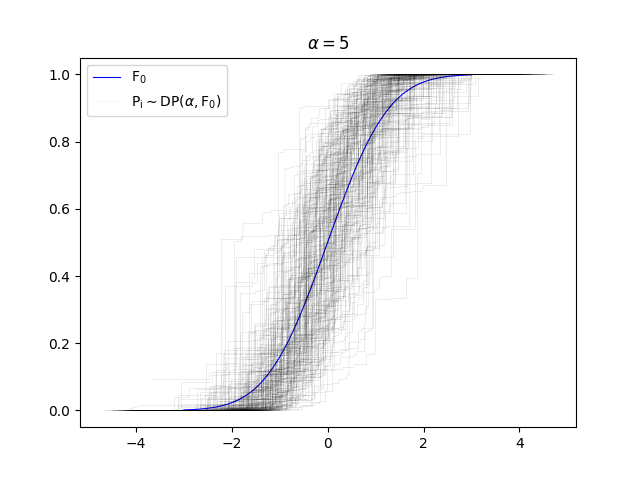
\includegraphics[width=0.48\linewidth]{ alpha5snorDP.png}
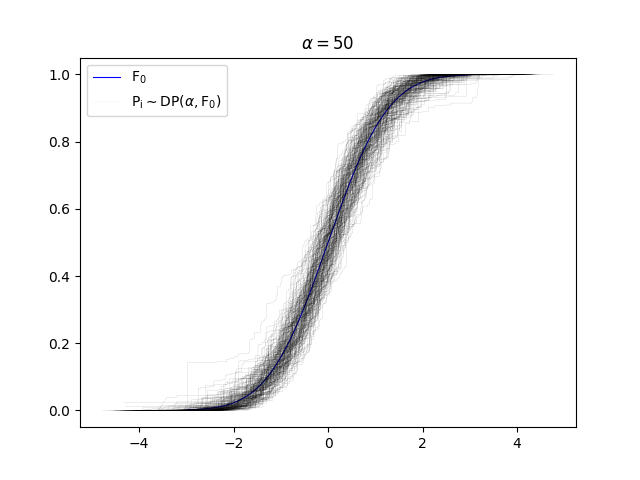
\includegraphics[width=0.48\linewidth]{ alpha50snorDP.png}
\caption{200 random measures sampled from $\mathrm{DP}(\alpha,\mathrm{F_{0}})$ where $\alpha = 5$ (left) and $50$ (right), $\mathrm{F_{0}} = N(0,1)$}
\label{fig:DP-alphalow-high}
\end{figure}

\paragraph{DPs for galaxy data-set}
We illustrate the application of Dirichlet processes for density estimation on a data set from the astronomy literature~\citep{roeder1990density}. The measurements are velocities at which galaxies in the Corona-Borealis region are moving away from our galaxy. If the galaxies are clustered, the velocity density will be multimodal, with clusters corresponding to modes. This happens to be the case, and the multi-modal nature is evident in the CDF of the data in Figure~\ref{fig:galaxy-dataset-DPprior/posterior} where the left and right regions of the CDF are almost flat, and most mass resides in the center. Starting with a $\mathrm{DP}(\alpha,N(0,1))$ prior, we obtain a DP posterior, and the spread of distributions sampled from the DP posterior (not shown) can be seen as confidence-set of the density estimate through Dirichlet process. 


\begin{figure}[h]
\centering
\includegraphics[width=0.6\linewidth]{Galaxy-data-example-DP-posterior.png}
\caption{A random measure sampled from DP prior, DP posterior compared against original galaxy dataset distribution.}
\label{fig:galaxy-dataset-DPprior/posterior}
\end{figure}




\section{DPPS for a Gaussian bandit}
\label{sec:DPPS-Gaussian-bandit}

\begin{figure}[H]
\centering
\includegraphics[width=0.55\linewidth]{ Bandit_Normal_unknown_mean_variance_DPPS_UCB.pdf}
\caption{DPPS for a challenging Gaussian bandit setting}
\label{fig:DPPS_Gaussian-bandit}
\end{figure}

A challenging  bandit setting is that of Gaussian bandit environment with both mean and variance of the underlying Gaussian distribution as unknown~\citep{cowan2018normal} to the bandit algorithm. Here we exhibit performance of DPPS in such a 7 arm Gaussian bandit environment $\{N(\mu_{k},\sigma_{k})\}_{k=1}^{K=7}$. The mean and variance of Gaussian bandit arms are sampled independently from a Gaussian such that $\mu_{k} \sim N(0,0.5)$  and $\sigma_{k} = |\psi_{k}|, \psi_{k} \sim N(0,0.5)$. Cumulative Regret averaged over 100 runs on one of the sampled instance of bandit environment is shown in Fig.~\ref{fig:DPPS_Gaussian-bandit}. Excellent performance of DPPS is evident. In this experiment, we chose $\alpha =2$, base measure of DP, $F_{0}$, as $N(0,0.5)$. 
 
\section{Choice of hyperparameters  in numerical experiments}
\label{sec:DPPSHyperparameters}

\begin{figure}[H]
\centering
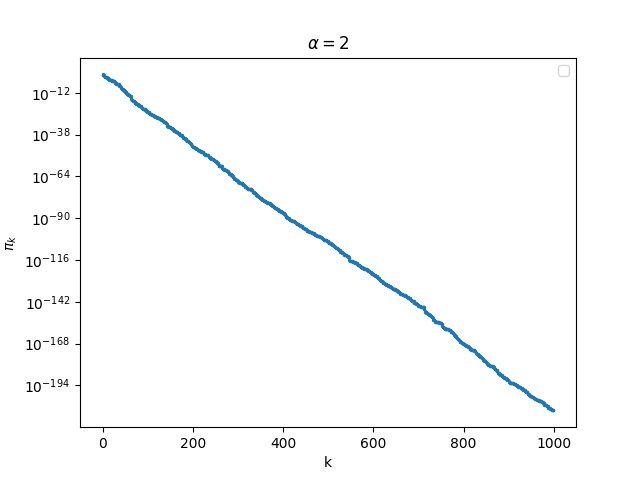
\includegraphics[width=0.48\linewidth]{ alpha-2-pi_k-k.png}
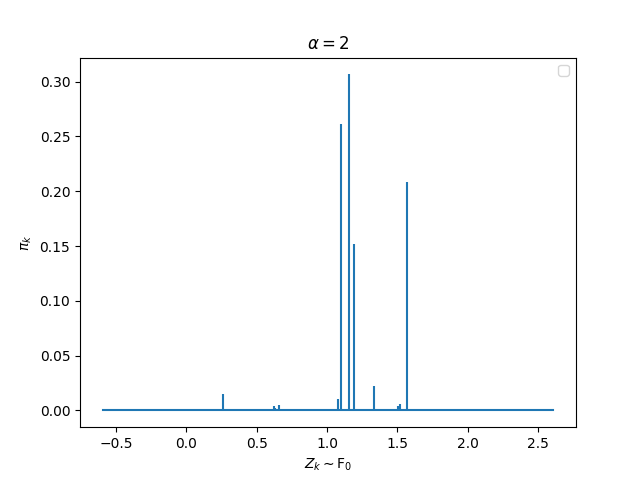
\includegraphics[width=0.48\linewidth]{ pi_k-Z_k-alpha-2.png}
\caption{Plot of first 1000 stick-breaking probability measure weights, $\pi_{k}$, for $\mathrm{DP}(\alpha=2,F_{0})$ with k (left) and with $Z_{k}\sim F_{0} (= N(0,1)$ (right)}
\label{fig:DP-alpha=2}
\end{figure}

\begin{figure}[H]
\centering
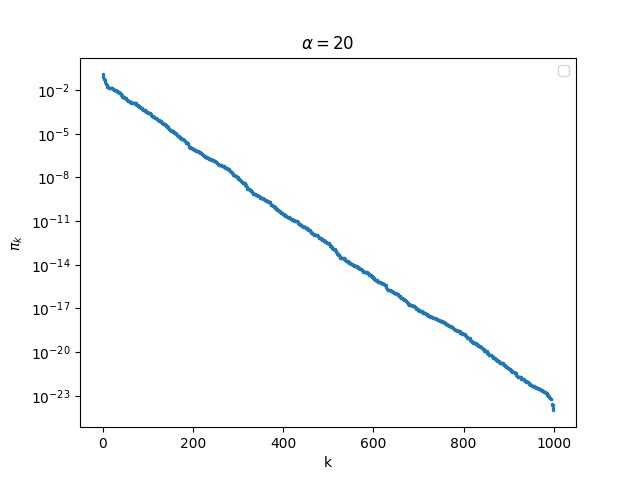
\includegraphics[width=0.48\linewidth]{ alpha20-pi_k-k.png}
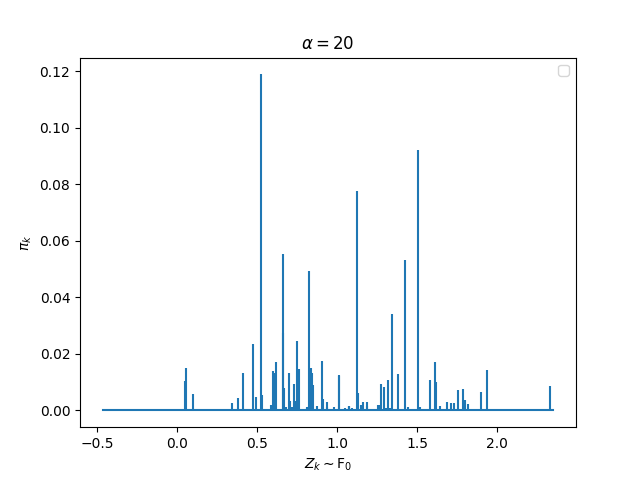
\includegraphics[width=0.48\linewidth]{ alpha-20-pi_k-Z_k.png}
\caption{Plot of first 1000 stick-breaking probability measure weights, $\pi_{k}$, for $\mathrm{DP}(\alpha=20,F_{0})$ with k (left) and with $Z_{k}\sim F_{0} (= N(0,1)$ (right)}
\label{fig:DP-alpha=20}
\end{figure}


Two hyperparameters in DPPS are $\alpha$ (concentration parameter) and $k_t$ (i.e. truncation level) in the stick breaking representation of DP prior (not the posterior), DP$(\alpha,F_{0})$.  We used $\alpha =2$ and $k_t = 100$ in all the experiments. Note that the choice of $\alpha$ directly influences the choice of $k_t$. This is because the number of weights $q_{i}$ in the stick breaking representation, $\sum q_{i} \delta_{x_{i}}$, carrying significant probability mass increase with increase in $\alpha$ ($V_{i}\sim$ Beta$(1,\alpha)$), and for higher $\alpha$ one needs to increase $k_t$.  For example, with $\alpha = 20$, we took $k_t =300$, and we got similar results, with a slight increase in computation cost though. An easy way to determine $k_t$ is to plot the stick breaking weights and remove stick breaking weights that are below a certain threshold (we chose $10^{-10}$ randomly). This relationship between $\alpha$ and stick breaking probability weights, $q_{i}$, can be seen in a simple example of $\mathrm{DP}(\alpha, F_{0})$ as shown in figs.~\ref{fig:DP-alpha=2}  and ~\ref{fig:DP-alpha=20}. Whereas for lower value of $\alpha$ only few weights have significant mass, for higher $\alpha$ the weights are more evenly spread compared to lower $\alpha$ case. 

\paragraph{Choice of base measure, $F_{0}$, of DP prior}

For choosing, $F_{0}$, the tail of the underlying reward distribution and a fact on the support of DPs is important. 
 
\begin{lemma}[Support of DPs, see~\citep{ghosal2010dirichlet}] In the \textit{weak topology}, the support of DP$(\alpha,F_{0})$ is characterized as all probability measures $P^\star$ whose supports are contained in that of $F_{0}$
\end{lemma}

Thus, choosing Beta(1,1) for a bandit problem with $\sigma = 10$, subGaussian noise is not a good idea. Similarly, theorem~\ref{thm:Bayesian-regret-DPPS} on Bayesian regret of DPPS, shows that choosing $F_{0}$ with $\sigma$-subGaussian tails corresponding to tails of the reward noise guarantees order optimal regret bounds.



\section{Running costs of DPPS}
\label{sec:computational-complexity-DPPS-NPTS}

Here we detail the computational costs associated to a single-arm in each round. Let $n$ denote the number of observations for the arm. The important consideration in quantifying the running cost of DPPS is to scrutinize the posterior update step,
\beqa
\label{eq:multi-step-posterior-appendix}
Q_{n} &=& V_{n}\delta_{X_{n}} + \sum_{i=1}^{n-1}\left[V_{i}\prod_{j=i+1}^{n}(1-V_{j})\right]\delta_{X_{i}} + \left[\prod_{i=1}^{n}(1-V_{i})\right] Q_{0}
\eeqa


Here, one needs to sample $n$ beta random variables and have $\mathcal{O}(n)$ multiplications of these random variables, one for each of the past observations. Thus the running cost of DPPS is $\mathcal{O}(n)$ for each arm. DPPS also incurs a fixed memory and computational cost of $\mathcal{O}(K)$, sampling a DP prior, $Q_{0}$, where $K$ is the truncation level of the DP prior. Clearly, this additional but constant (in number of rounds and memory) cost is the difference between computational complexities of DPPS and NPTS (which needs similar $\mathcal{O}(n)$ multiplications between $\bf{X_{n}}$ and $\bf{W_{n}}\sim\mathrm{Dir}(n;1,. . .,1)$ random variables), and arises because of additional flexibility of DPPS in incorporating prior knowledge. 








%\section{Valid posteriors and optimality of DPPS}\label{sec:valid-posteriors}
%\oam{Do you use $a*$ or $a^\star$ for optimal arm notation?}

%The above analysis of ~\citep{russo2016information} was carried out for Thompson-sampling, which relies on the application of Bayes rule to derive the posterior distribution of optimal actions, $\alpha_{t}(a^\star) = P_{t}(A^\star=a^\star)$ and chooses actions according to the policy $\pi_{t}(a) = \alpha_{t}(a)$. Scrutinizing the proof, we observe, however, that this requirement of $\alpha_{t}(a)$ being based on Bayes rule is nowhere required in the proof above. Rather, It was implicit in their proof that $P(A^\star=a)$ is a \textit{valid} Bayesian posterior which is the natural choice under the umbrella of decision theory~\citep{north1968tutorial}. Thus, the results in~\citep{russo2016information} actually hold for any algorithm that utilizes \textit{valid} Bayesian posterior update scheme.    Recall from Section~\ref{sec:Bayesian-framework} that it's not possible to use Bayes rule for most non-parametric priors, and in general the conjugate posterior-prior relationship is the \textit{valid} Bayesian posterior update scheme for non-parametric priors. Since DPPS utilizes this conjugate prior/posterior relationship in DP posteriors to derive $P(A^\star=a)$, our simple argument leads us to the following result, 

%\begin{thm}\label{thm:Equivalence-of-TS-DPPS}
%The optimality guarantees of DPPS are equivalent to that of Thompson-sampling in the Bayesian regret framework.
%\end{thm}



%Using Theorem~\ref{thm:Equivalence-of-TS-DPPS} and Theorem~\ref{thm:Bayesian-regret-MAB-TS}, we obtain,

%\begin{thm}
%\[\E\left[\mathrm{Regret}(T,\pi^{DPPS})\right] \le \sigma\sqrt{|\mathcal{A}|\log(|\mathcal{A}|)T}\]
%\end{thm}

%where the expectation averages over the randomness introduced by the DP prior and the policy. When $\sigma = \sqrt{1/2}$ one recovers result for rewards bounded between 0 and 1 (stated in our main paper.)



\section{Further related work}
\label{sec:Related works}

To the best of our knowledge, Dirichlet Processes in the context of bandits were first used in ~\citep{clayton1985bayesian} to study a version of the single-arm  Gittin's index problem, when the probability distribution of the arm is assumed to be DP distributed. Use of Bootstrapping for Thompson sampling seems to have appeared first in \cite{eckles2014thompson}, which was further improved and made more systematic in ~\citep{osband2015bootstrapped} where the authors also showed equivalence of Bootstrap-Thompson sampling (for Bernoulli-bandits) and Thompson sampling with Beta/Bernoulli priors in an exact sense, and speculated this equivalence for a wide class of bandit-environments if a proper mechanism for generating \textit{artifical history} (or prior information) could be identified. As shown in the current paper, DPPS provides a neat and principled mechanism for incorporating prior information (or gnerating artificial history), and generalizes this equivalence. Non-Parametric Thompson sampling (NPTS) and Multinomial Thompson Sampling (TS) were introduced in~\citep{riou2020bandit} without highlighting any concrete Bayesian connection of the former algorithm. NPTS was adapted for robustness in ~\citep{baudry2021optimality}. Some discussions concerning Bayesian interpretation of NPTS using DPs appeared in \cite{belomestny2023sharp} who provided a refined analysis of Multinomial TS.  Aligning towards non-Bayesian side,  a sample mean based algorithm guaranteeing $O(\log N)$ instance-dependent regret appeared in \cite{agrawal1995sample}, a sub-sampling based algorithm was reported in \cite{baransi2014sub} and analyzed for a two-arm bandit setting; a nonparametric Bootstrap based algorithm  was reported in \cite{kveton2019garbage}, and regret bounds derived for a Bernoulli bandit environment.


\section{Technical derivations}
\label{sec:Proofs}

This section gives proofs of lemmas in the main paper extracted here for completion from ~\citep{russo2016information}


\subsection{Proof of Lemma~\ref{fact:Bayesian-regret-information-ratio}}

\begin{lemma}\label{prop: regret bound}
For any $T\in \mathbb{N}$, if $\Gamma_t \leq \overline{\Gamma}$ almost surely for each $t \in \{1,..,T\}$,  
$$\E \left[{\rm Regret}(T, \pi^{\rm TS})  \right] \leq  \sqrt{\overline{\Gamma} \H(\alpha_1) T}.$$
\end{lemma}
\begin{proof} Recall that $\E_{t}[\cdot] = \E[\cdot | \hist]$ and we use $I_{t}$ to denote mutual information evaluated under the base measure $\Prob_{t}$. Then,
%Taking the expectation of both sides of \eqref{eq: rewrite regret in terms of info gain} in Proposition \ref{prop: rewrite regret} and summing over $t$ shows
\begin{eqnarray*}
\E \left[{\rm Regret}(T, \pi^{\rm TS})  \right] \overset{(a)}{=} \mathbb{E} \sum_{t=1}^{T} \E_{t} \left[ R_{t, A^\star} -R_{t,A_t} \right]  &=& \mathbb{E}\sum_{t=1}^{T} \sqrt{\Gamma_{t} I_{t}\left( A^\star ; (A_t, R_{t, A_t})  \right)} \\ 
&\leq& \sqrt{\overline{\Gamma}}\left( \mathbb{E} \sum_{t=1}^{T} \sqrt{I_{t}\left( A^\star ; (A_t, R_{t, A_t})  \right)} \right) \\
&\overset{(b)}{\leq}& \sqrt{\overline{\Gamma}T \mathbb{E} \sum_{t=1}^{T} I_{t}\left( A^\star ; (A_t, R_{t, A_t})  \right)},
\end{eqnarray*}
where (a) follows from the tower property of conditional expectation, and (b) follows from the Cauchy-Schwartz inequality. We complete the proof by showing that expected information gain cannot exceed the entropy of the prior distribution. For the remainder of this proof, let $Z_t = (A_t, R_{t,A_t})$. Then, using tower rule of conditional expectations we have,
\[
 {\E_{t}}\left[ I_{t}\left( A^\star ;Z_t \right) \right] =  I\left( A^\star ; Z_t | Z_1,...,Z_{t-1}  \right),
\]
and therefore,
\begin{eqnarray*}
\mathbb{E}\sum_{t=1}^{T} I_{t}\left( A^\star ; Z_t  \right) =  \sum_{t=1}^{T} I\left( A^\star ; Z_t | Z_1,...,Z_{t-1}  \right)
&\overset{(c)}{=}&  I\left(A^\star \, ;\,  Z_1,...Z_{T}    \right) \\ 
&=& \H(A^\star) - \H(A^\star | Z_1,...Z_{T}) \\
&\overset{(d)}{\leq}&  \H(A^\star),
\end{eqnarray*}
where (c) follows from the chain rule for mutual information, and (d) follows from the non-negativity of entropy.
\end{proof}

\subsection{Proof of Lemma~\ref{fact:KL-var-X}}

\begin{proof}
Define the random variable $X(t)=R_{t,a}- \E_{t}\left[ R_{t,a}\right]$. Then, for arbitrary $\lambda \in \mathbb{R}$, applying Fact \ref{fact:KL-var} to $\lambda X$ yields
\begin{eqnarray*}
\KL \left(\Prob_{t}\left( R_{t,a}  | A^\star=a^\star \right) \, || \, \Prob_{t}( R_{t,a})\right) &\geq& \lambda \E_{t}\left[X | A^\star=a^\star \right] - \log \E_{t} \left[ \exp\{\lambda X \} \right]\\
&= & \lambda \left( \E_{t}[R_{t,a}| A^\star=a^\star]- \E_{t}\left[ R_{t,a}\right] \right)- \log \E_{t} \left[ \exp\{\lambda X \}\right] \\
&\geq&\lambda \left( \E_{t}[R_{t,a}| A^\star=a^\star]- \E_{t}\left[ R_{t,a}\right] \right) - (\lambda^2 \sigma^2 /2).
\end{eqnarray*}
Maximizing over $\lambda$ yields the result. 
\end{proof}

\subsection{Proof of Lemma~\ref{fact:Information-ratio-MAB-for-sub-gaussian-rewards}}

\begin{proof}   
\begin{eqnarray*}
\E_{t} \left[ R_{t,A^\star} - R_{t,A_{t}}\right]^2 &\overset{(a)}{=}&  \left(\sum_{a\in \A} \Prob_{t}(A^\star=a) \left( \E_{t}\left[R_{t,a} | A^\star=a \right] - \E_{t}[R_{t,a}]\right) \right)^2 \\
&\overset{(b)}{\leq}& |\A|  \sum_{a\in \A} \Prob_{t}(A^\star=a)^2 \left( \E_{t}\left[R_{t,a} | A^\star=a \right] - \E_{t}[ R_{t,a}]\right)^2    \\
&\leq& |\A|  \sum_{a, a^\star \in \A} \Prob_{t}(A^\star=a)\Prob_{t}(A^\star=a^\star) \left( \E_{t}\left[R_{t,a} | A^\star=a^\star \right] - \E_{t}[ R_{t,a}]\right)^2   \\
&\overset{(c)}{\leq}& \frac{|\A|}{2} \sum_{a, a^\star \in \A} \Prob_{t}(A^\star=a)\Prob_{t}(A^\star=a^\star){\KL}\left(\Prob_{t}(R_{t,a} | A^\star = a^\star)   \,\, || \,\, \Prob_{t}(R_{t,a})  \right)  \\
&\overset{(d)}{=}& \frac{|\A| I( A^\star ; R_{t,A_{t}})}{2}
\end{eqnarray*}
where (b) follows from the Cauchy--Schwarz inequality, (c) follows from Fact \ref{fact:KL-var-X}, and (a) follows from Eq.\ref{Eq:Regret-decomposition}and (d) from the standard definition of mutual-information. 
\end{proof}





\end{document}
